\chapter{Markov Chains (draft)}

\section{Definition and Basic Facts}

\section{Class Division}

\section{Markov Chain Equations}

\section{Strong Markov Property}

\section{Recurrent and Transience}

%%%%%%%%%%%%%%%%%%%%%%%%%%%%%%%%%%%%%%%%%%%%%%%%%%%%%%










%%%%%%%%%%%%%%%%%%%%%%%%%%%%%%%%%%%%%%%%%%%%%%%%%%%%%%

\section{Exercises}

\begin{problem}
The village green is ringed by a fence with $N$ fenceposts, labelled $0,1,\dots,N-1$. The village idiot is given a pot of paint and a brush, and started at post 0 with instructions, 1 paint all the posts. He paints post 0, and then chooses one of the two nearest neighbours, 1 or $N-1$, with equal probability, moving to the chosen post and painting it. After painting a post, he chooses with equal probability one of the two nearest neighbours, moves there and paints it (regardless of whether it is already painted). Find the distribution of the last post unpainted. (What is the expected time to paint all the fence?)
\end{problem}

\begin{solution}
If $k$ is the last painted fence, there are 2 ways to reach it, from $k-1$ and $k+1$. We can find these 2 probabilities separately.

\centertexdraw{

\drawdim in

\def\bdot {\fcir f:0 r:0.025 }
\arrowheadtype t:F \arrowheadsize l:0.08 w:0.04
\linewd 0.01 \setgray 0

\move (0 0)\bdot
\move (0.5 0)\bdot
\move (1.0 0)\bdot
\htext(1.4 0){$\dots$}
\move (2 0)\bdot
\htext(2.4 0){$\dots$}
\move (3 0)\bdot
\move (3.5 0)\bdot
\move (4.0 0)\bdot

\move (0.25 -0.2) \larc r:0.3 sd:45 ed:135
\move (0.25 0.1) \avec(0.24 0.1)
\move (0.25 0.2) \larc r:0.3 sd:225 ed:315
\move (0.25 -0.1) \avec(0.26 -0.1)

\move (0.75 -0.2) \larc r:0.3 sd:45 ed:135
\move (0.75 0.1) \avec(0.74 0.1)
\move (0.75 0.2) \larc r:0.3 sd:225 ed:315
\move (0.75 -0.1) \avec(0.76 -0.1)

\move (3.25 -0.2) \larc r:0.3 sd:45 ed:135
\move (3.25 0.1) \avec(3.24 0.1)
\move (3.25 0.2) \larc r:0.3 sd:225 ed:315
\move (3.25 -0.1) \avec(3.26 -0.1)

\move (3.75 -0.2) \larc r:0.3 sd:45 ed:135
\move (3.75 0.1) \avec(3.74 0.1)
\move (3.75 0.2) \larc r:0.3 sd:225 ed:315
\move (3.75 -0.1) \avec(3.76 -0.1)

\htext (-0.03 -0.3){$k$}
\htext (0.37 -0.3){$k-1$}
\htext (1.97 -0.3){$0$}
\htext (2.97 -0.3){$-(N-k-1)$}
\htext (3.97 -0.3){$-(N-k)$}
}

First, from $k-1$, the probability is
\be
\pro_0(\text{hit $-(N-k-1)$ before $k$})\ \pro_{k-1}(\text{hit $k$ before $-(N-k)$})
\ee

We know
\be
\pro_i(\text{hit $-(N-k-1)$ before $k$}) = \frac{k-i}{N-1},\quad \pro_i(\text{hit $k$ before $-(N-k)$}) = \frac{i+N-k}{N}
\ee

Thus,
\be
\pro(\text{painter reach $k$ from $k-1$}) = \frac{k}{N-1} \frac{1}{N} = \frac k{N(N-1)}.
\ee

Similarly,
\be
\pro(\text{painter reach $k$ from $k+1$}) = \frac{N-k}{N-1} \frac{1}{N} = \frac {N-k}{N(N-1)}.
\ee

Hence
\beast
\pro(\text{$k$ is the last painted fence}) & = & \pro(\text{painter reach $k$ from $k-1$}) + \pro(\text{painter reach $k$ from $k+1$}) \\
& = & \frac k{N(N-1)} + \frac {N-k}{N(N-1)} = \frac 1{N-1}.
\eeast

We define $h_i$ the probability that the painter hits $-(N-k-1)$ before $k$ from $i$ and
\beast
\tilde{p}_{ij} & = & \pro(X_1=j|X_0=i,\text{hit $-(N-k-1)$ before $k$}) \\
& = & \frac {\pro(X_1=j,\text{hit $-(N-k-1)$ before $k$}|X_0=i)}{\pro(\text{hit $-(N-k-1)$ before $k$}|X_0=i)} \\
& = & \frac {\pro(\text{hit $-(N-k-1)$ before $k$}|X_1=j,X_0=i)\pro(X_1=j|X_0=i)}{h_i} \\
& = & \frac {\pro(\text{hit $-(N-k-1)$ before $k$}|X_1=j)\pro(X_1=j|X_0=i)}{h_i} \\
& = & \frac{h_j}{h_i}p_{ij}
\eeast

Then we calculate
\be\left\{
\ba{l}
\tilde{p}_{i,i+1} = \frac {k-i-1}{k-i}p_{i,i+1} = \frac{k-i-1}{2(k-i)} \\
\\
\tilde{p}_{i,i-1} = \frac {k-i+1}{k-i}p_{i,i+1} = \frac{k-i+1}{2(k-i)}
\ea\right.
\ee

The expected time starting at $i$, $T_i$ is given by
\be
\left\{
\ba{l}
T_{k-1} = 1+ T_{k-2}\\
\vdots\\
T_i = 1+ \frac{k-i+1}{2(k-i)} T_{i-1} + \frac{k-i-1}{2(k-i)} T_{i+1}\\
\vdots\\
T_{-(N-k-2)} = 1 + \frac{N-3}{2(N-2)} T_{-(N-k-3)}
\ea\right.\ \ra \
\left\{\ba{l}
2T_{k-1} = 2+ 2T_{k-2}\\
\vdots\\
2(k-i) T_i = 2(k-i) + (k-i+1)T_{i-1} + (k-i-1) T_{i+1}\\
\vdots\\
2(N-2) T_{-(N-k-2)} = 2(N-2) + (N-3) T_{-(N-k-3)}
\ea\right.
\ee

Let $U_i = (k-i)T_i$
\be
\left\{\ba{l}
2U_{k-1} = 2+ U_{k-2}\\
\vdots\\
2U_i = 2(k-i) + U_{i-1} + U_{i+1}\\
\vdots\\
2U_{-(N-k-2)} = 2(N-2) + U_{-(N-k-3)}
\ea\right.
\ \ra \ U_{k-1} + U_{-(N-k-2)} = 2\sum^{N-2}_{i=1} i = (N-1)(N-2)
\ee

Also, we have
\be
\left\{\ba{l}
2U_{k-1} = 2+ U_{k-2}\\
3U_{k-2} = 10 + 2U_{k-3}\\
4U_{k-3} = 28 + 3U_{k-4}\\
\vdots\\
(k-i+1)U_i = 2\sum^{k-i}_{j=1}j^2 + (k-i)U_{i-1} \\
\vdots\\
(N-3)U_{-(N-k-4)} = 2\sum^{N-4}_{j=1}j^2 + (N-4)U_{-(N-k-3)}\\
\\
(N-2)U_{-(N-k-3)} = 2\sum^{N-3}_{j=1}j^2 + (N-3)U_{-(N-k-2)}
\ea\right.
\ee

Thus,
\be
\ \ra \ \left\{\ba{l}
(N-2)U_{-(N-k-3)} = \frac {(N-3)(N-2)(2N-5)}{3} + (N-3)U_{-(N-k-2)}\\
2U_{-(N-k-2)} = 2(N-2) + U_{-(N-k-3)}
\ea\right. \ \ra \
\left\{\ba{l}
U_{-(N-k-2)} = \frac {(N-2)(2N-3)}{3}\\
U_{-(N-k-3)} = \frac {4(N-2)(N-3)}{3}
\ea\right.
\ee

and $U_{k-1} = \frac {N(N-2)}{3}$. Thus, we have
\be
U_i = \frac{k-i}{3}\left[(N-1)^2 - (k-i)^2\right] \ \ra \ T_i = \frac 13\left[(N-1)^2 - (k-i)^2\right] \ \ra \ T_0 = \frac 13\left[(N-1)^2 - k^2\right]
\ee

Similarly, expected time from $-(N-k-1)$ to $k$ is
\be
T_{-(N-k-1)}' = \frac {N^2-1}{3}
\ee

Thus, the painter approach $k$ from $k-1$ with probability $\frac{k}{N}$ and expected time
\be
\frac 13\left[(N-1)^2 - k^2\right] + \frac {1}{3}(N^2-1)= \frac 13\lob 2N^2 -2N- k^2\rob
\ee

Similarly, the painter approach $k$ from $k+1$ with probability $\frac{N-k}{N}$ and expected time
\be
\frac 13\lob 2N^2 -2N- (N-k)^2\rob
\ee

Thus, the expected time to reach the last fence $k$ is
\bea
& & \frac 1{3N}\lob 2kN^2 -2kN- k^3 + 2(N-k)N^2 -2(N-k)N- (N-k)^3\rob \nonumber\\
& = & \frac 1{3N}\lob 2N^3 -2N^2- k^3 - (N-k)^3\rob = \frac 13\lob 2N^2 - 2N - (N^2-3kN +3k^2) \rob\nonumber\\
& = & \frac 13\lob N^2 - 2N + 3kN - 3k^2 \rob
\eea

Since the distribution is uniform, we have the total expected time
\bea
& & \frac 13\lob N^2 - 2N\rob + \frac{1}{N-1}\lob N\sum^{N-1}_{k=1}k - \sum^{N-1}_{k=1}k^2 \rob \nonumber\\
& = & \frac 13\lob N^2 - 2N\rob + \frac12 N^2 - \frac 16 N(2N-1)\nonumber\\
& = & \frac 12 N(N-1).
\eea
\end{solution}

\begin{problem}
The (symmetric) random walk $X_0$ starts from 0. What's the probability that it hits $N$ before returning 0? Assume $N=10$, what's the probability that it hits $10$ before returning 0 and hits 10 with 20 steps?
\end{problem}

\begin{solution}
If it jumps to -1, it will hit 0 before $N$. So with probability $\frac 12$, it hits 1 first. We consider the random walk starting at 1. Let $h_i$ be the probability that it hits 10 before 0 starting from $i$. From the OST, we have
\be
h_i = \frac iN.
\ee

Then we have the new probability
\beast
\wh{p}_{ij} = \pro(X_1=j|X_0=i,\text{hits $10$ before $0$}) & = & \frac{\pro(X_1=j,\text{hits $10$ before $0$}|X_0=i)}{\pro(\text{hits $10$ before $0$}|X_0=i)} \\
& = & \frac{\pro(\text{hits $10$ before $0$}|X_0=i,X_1=j)\pro(X_1=j|X_0 =i)}{\pro(\text{hits $10$ before $0$}|X_0=i)}\\
& = & \frac{\pro(\text{hits $10$ before $0$}|X_1=j)\pro(X_1=j|X_0 =i)}{\pro(\text{hits $10$ before $0$}|X_0=i)}  = \frac{h_j}{h_i}p_{ij}
\eeast

So we have
\be
\wh{p}_{i,i+1} = \frac{h_{i+1}}{h_i}p_{i,i+1} = \frac {\frac{i+1}{10}}{\frac i{10}}\frac 12 = \frac {i+1}{2i}, \quad \quad \wh{p}_{i,i-1} = \frac {i-1}{2i},\quad\quad i = 1,\dots,9.
\ee

Then Let $F_i = \E\bb{z^\tau|X_0=i,\text{hits $10$ before $0$}}$ be the probability generating function where $\tau$ is the stopping time. Then
\be
F_i = z\bb{\wh{p}_{i,i+1} F_{i+1} + \wh{p}_{i,i-1} F_{i-1}} \ \ra \ 2iF_i = z \bb{(i+1) F_{i+1} + (i-1) F_{i-1}}
\ee

Let $G_i = iF_i$, then
\be
2G_i = z \bb{G_{i+1} + G_{i-1}} \ \ra \ zG_{i+1} -2G_i + zG_{i-1} = 0
\ee
which has the auxiliary equation
\be
z a^2 - 2a + z = 0 \ \ra \ a = \frac{2 \pm \sqrt{4-4z^2}}{2z} = \frac {1\pm \sqrt{1-z^2}}z \ \ra \ G_i = A\bb{\frac {1+ \sqrt{1-z^2}}z}^i + B\bb{\frac {1- \sqrt{1-z^2}}z}^i.
\ee

With the boundary condition $G_0 = 0$ and $G_{10} = 10$, we have

\be
G_i = \frac{10}{\bb{\frac {1+ \sqrt{1-z^2}}z}^{10} - \bb{\frac {1- \sqrt{1-z^2}}z}^{10}}\bb{\bb{\frac {1+ \sqrt{1-z^2}}z}^i - \bb{\frac {1- \sqrt{1-z^2}}z}^i}
\ee

Then
\be
F_i = \frac{10}{i \bb{\bb{\frac {1+ \sqrt{1-z^2}}z}^{10} - \bb{\frac {1- \sqrt{1-z^2}}z}^{10}}}\bb{\bb{\frac {1+ \sqrt{1-z^2}}z}^i - \bb{\frac {1- \sqrt{1-z^2}}z}^i}
\ee
particularly, we want to know
\beast
F_1 & = & \frac{10 z^9\bb{\bb{1+ \sqrt{1-z^2}} - \bb{1- \sqrt{1-z^2}}}}{\bb{1+ \sqrt{1-z^2}}^{10} - \bb{1- \sqrt{1-z^2}}^{10}} = \frac{20 z^9 \sqrt{1-z^2}}{\bb{1+ \sqrt{1-z^2}}^{10} - \bb{1- \sqrt{1-z^2}}^{10}}\\
& = & \frac{10 z^9 \sqrt{1-z^2}}{10 (1-z^2)^{\frac 12} + 120 (1-z^2)^{\frac 32} + 252 (1-z^2)^{\frac 52} + 120 (1-z^2)^{\frac 72}+10 (1-z^2)^{\frac 92}}\\
& = & \frac{10 z^9}{10 + 120 (1-z^2) + 252 (1-z^2)^2 + 120 (1-z^2)^3 +10 (1-z^2)^4}\\
& = & \frac{10 z^9}{10 + 120 -120 z^2 + 252 - 504z^2 + 252 z^4 + 120 - 360z^2 + 360z^4 -120z^6 +10 - 40z^2 + 60z^4 - 40 z^6 + 10z^8}\\
& = & (10 z^9)\left/\bb{512 -1024 z^2 + 672 z^4 - 160z^6 + 10z^8}\right.\\
& = & 10\left/\bb{\frac{512}{z^9} -\frac{1024}{z^7} + \frac{672}{z^5} - \frac{160}{z^3} + \frac{10}{z}}\right.
\eeast

Thus, we know the first item of $F_1(z)$ is $\frac1{512}z^9$ then assume
\be
F_1 (z) = \frac 1{2^9} z^9 + A z^{11} + \dots
\ee
Then the coefficient of term $z^2$ of $\frac {F_1}{10} \bb{\frac{512}{z^9} -\frac{1024}{z^7} + \frac{672}{z^5} - \frac{160}{z^3} + \frac{10}{z}}$ must be
\be
0 = A z^{11} \frac{512}{z^9} - \frac 1{2^9} z^9 \frac{1024}{z^7} = z^2\bb{512A - 2} \ \ra \ A = \frac 1{256}
\ee

then assume

\be
F_1 (z) = \frac 1{2^9} z^9 + \frac 1{2^8}z^{11} + A z^{13} \dots
\ee
Then the coefficient of term $z^4$ of $\frac {F_1}{10} \bb{\frac{512}{z^9} -\frac{1024}{z^7} + \frac{672}{z^5} - \frac{160}{z^3} + \frac{10}{z}}$ must be
\be
0 = A z^{13} \frac{512}{z^9} - \frac 1{2^8} z^{11} \frac{1024}{z^7} +  \frac 1{2^9} z^9 \frac{672}{z^5} = z^4\bb{512A - 4 + \frac {21}{16}} \ \ra \ A = \frac {43}{2^{13}}
\ee

then assume

\be
F_1 (z) = \frac 1{2^9} z^9 + \frac 1{2^8}z^{11} + \frac {43}{2^{13}} z^{13} + A z^{15} \dots
\ee
Then the coefficient of term $z^6$ of $\frac {F_1}{10} \bb{\frac{512}{z^9} -\frac{1024}{z^7} + \frac{672}{z^5} - \frac{160}{z^3} + \frac{10}{z}}$ must be
\be
0 = A z^{15} \frac{512}{z^9} - \frac {43}{2^{13}} z^{13} \frac{1024}{z^7} +  \frac 1{2^8}z^{11} \frac{672}{z^5} - \frac 1{2^9} z^9 \frac{160}{z^3} = z^6\bb{512A - \frac{43}8 + \frac {21}{8} - \frac 5{16}} \ \ra \ A = \frac {49}{2^{13}}
\ee

then assume
\be
F_1 (z) = \frac 1{2^9} z^9 + \frac 1{2^8}z^{11} + \frac {43}{2^{13}} z^{13} + \frac {49}{2^{13}} z^{15} + A z^{17} \dots
\ee
Then the coefficient of term $z^8$ of $\frac {F_1}{10} \bb{\frac{512}{z^9} -\frac{1024}{z^7} + \frac{672}{z^5} - \frac{160}{z^3} + \frac{10}{z}}$ must be
\beast
0 & = & A z^{17} \frac{512}{z^9} - \frac {49}{2^{13}} z^{15}  \frac{1024}{z^7} + \frac {43}{2^{13}} z^{13}  \frac{672}{z^5} - \frac 1{2^8}z^{11}  \frac{160}{z^3} + \frac 1{2^9} z^9 \frac{10}{z} \\
& = & z^8\bb{512A - \frac{49}8 + \frac {903}{2^8} - \frac{160}{2^8} + \frac 5{2^8}} \ \ra \ A = \frac {205}{2^{15}}
\eeast

then assume

\be
F_1 (z) = \frac 1{2^9} z^9 + \frac 1{2^8}z^{11} + \frac {43}{2^{13}} z^{13} + \frac {49}{2^{13}} z^{15} + \frac {205}{2^{15}} z^{17} + A z^{19} \dots
\ee
Then the coefficient of term $z^{10}$ of $\frac {F_1}{10} \bb{\frac{512}{z^9} -\frac{1024}{z^7} + \frac{672}{z^5} - \frac{160}{z^3} + \frac{10}{z}}$ must be
\beast
0 & = & A z^{19} \frac{512}{z^9} - \frac {205}{2^{15}} z^{17} \frac{1024}{z^7} + \frac {49}{2^{13}} z^{15}  \frac{672}{z^5} - \frac {43}{2^{13}} z^{13}  \frac{160}{z^3} + \frac 1{2^8}z^{11}  \frac{10}{z} \\
& = & z^{10}\bb{512A - \frac{205}{2^5} + \frac {1029}{2^8} - \frac{215}{2^8} + \frac {10}{2^8}} \ \ra \ A = \frac {51}{2^{13}}
\eeast

Then the probability for random walk to hit 10 before 0 with 20 steps is
\be
\frac 12 \cdot \frac {51}{2^{13}} = \frac {51}{2^14} = 0.00311.
\ee

The probability to hit 10 before 0 less than or equal to 20 step is
\be
\frac 12 \bb{\frac 1{2^9} + \frac 1{2^8} + \frac {43}{2^{13}} + \frac {49}{2^{13}} + \frac {205}{2^{15}}+ \frac {51}{2^{13}}} = \frac {969}{2^{16}} = 0.0148.
\ee
\end{solution}



\begin{exercise}
Let $(X_n)_{n\geq 0}$ be a discrete-time $(\lm,P)$ Markov chain. Determine the conditions on the initial distribution $\lm$ and transition matrix $P$ under which random variables $X_0,X_1,\dots$ are independent and identically distributed, i.e.:
\be
\pro(X_0=i_0,\dots,X_n=i_n)=\prod^n_{j=1}\pro(X_0=i_j).
\ee

A particle moves among the vertices of a perfect polygon. Find if its positions $X_n,\ n\geq 0$, from a Markov chain under the following rules:

(a) the particle always moves clockwise with step one,

(b) at time $n=0$ the particle chooses at random one of the directions and then moves all the time in this direction with step one,

(c) the particle moves to the clockwise adjacent vertex with probability $p$ and to the anti-clockwise adjacent vertex with probability $q=1-p$,

(d) the particle moves as in (c), except for a single vertex, say $a_1$ from which it always returns to the vertex it came from.

Write down the corresponding transition matrices.
\end{exercise}

Solution. If $X_0,X_1,\dots$ are i.i.d., we have
\be
\pro(X_0=i,X_1=j) = \pro(X_0=i)\pro(X_1=j)\ \ra \ \lm_i p_{ij} = \lm_i\lm_j\ \ra \ p_{ij} = \lm_j, \quad\forall i:\lm_i\neq 0
\ee
with the above condition, we have
\be
\pro(X_0=i_0,\dots,X_n=i_n)=\prod^n_{j=1}\pro(X_0=i_j) =\lm_{i_0}p_{i_0i_1}\dots p_{i_{n-1}i_n} = \lm_{i_0}\lm_{i_1}\dots\lm_{i_n} = \prod^n_{j=1}\pro(X_0=i_j).
\ee

(a) It is a Markov chain and transition matrix is
\be
\lob
\ba{ccccc}
0 & 1 & 0 & \cdots & 0 \\
0 & 0 & 1 & \cdots & 0 \\
\vdots & \vdots & \vdots & \ddots & \vdots  \\
0 & 0 & 0 & \cdots & 1 \\
\ 1 \ \ & \ 0 \ \ & \ 0 \ \  &\  \cdots \ \  & \  0 \ \
\ea
\rob.
\ee

(b) It is not a Markov chain since
\be
\left\{\ba{l}
\pro(X_2=3|X_0=1,X_1=2) = 1\\
\\
\pro(X_2=3|X_0=3,X_1=2) = 0
\ea\right.
\ee

(c) It is a Markov chain and transition matrix is
\be
\lob
\ba{ccccc}
0 & p & 0 & \cdots & 1-p \\
1-p & 0 & p & \cdots & 0 \\
0 & 1-p & 0 & p & \vdots \\
\vdots & \vdots & \ddots & \ddots & \vdots  \\
\ p \ \ & \ 0 \ \ & \ \cdots \ \  &\  1-p \ \  & \  0 \ \
\ea
\rob.
\ee

(d) It is not a Markov chain since
\be
\left\{\ba{l}
\pro(X_2=1|X_0=1, X_1=a_1) = 1\\
\\
\pro(X_2=1|X_0=3, X_1=a_1) = 0
\ea\right.
\ee


\begin{exercise}
Let $B_1,B_2,\dots$ be disjoint events with $\cup^\infty_{n=1}B_n=\Omega$. Show that if $A$ is another event and $\pro (A|B_n)=p$ for all $n$ then $\pro (A)=p$. Deduce that if $X$ and $Y$ are discrete random variables then the following are equivalent:

(a) $X$ and $Y$ are independent;

(b) the conditional distribution of $X$ given $Y=y$ is independent of $y$.
\end{exercise}

Solution. Since $B_1,B_2,\dots$ are disjoint events,
\bea
\pro (A) & = & \pro (A|\Omega) = \pro (A|\cup^\infty_{n=1}B_n) = \frac{\pro(\cup^\infty_{n=1}B_n|A)\pro(A)}{\pro (\cup^\infty_{n=1}B_n)} = \pro(\cup^\infty_{n=1}B_n|A)\nonumber\\
& = & \sum^\infty_{n=1}\pro(B_n|A)\pro(A) = \sum^\infty_{n=1}\pro(A|B_n)\pro(B_n) = p\sum^\infty_{n=1}\pro(B_n) = p
\eea

(a)$\Rightarrow$(b):
\be
\pro(X=x,Y=y) = \pro(X=x)\pro(Y=y) \ \Rightarrow \ \pro(X=x|Y=y) = \pro(X=x)
\ee

(b)$\Rightarrow$(a): Let $A=\{X=x\}$, $B_n=\{Y=y\}$ for all $x,y\in \Omega$
\be
\pro(X=x|Y=y) = p_x \ \Rightarrow \ \pro(X=x) = p_x
\ee

Thus, (a) and (b) are equivalent.

\begin{exercise}
Show that if $(X_n)_{n\geq 0}$ is a discrete-time Markov chain with transition matrix $P$ and $Y_n=X_{kn}$, then $(Y_n)_{n\geq 0}$ is a Markov chain with transition matrix $P^k$.
\end{exercise}

Solution. By the strong Markov property, conditional on $X_m=i$, $(X_{m+n})_{n\geq 0}$ is a Markov chain with transition matrix $P$ and independent of $X_0,X_1,\dots,X_{m-1}$.
\bea
& &\pro(Y_{n+1}=i_{n+1}|Y_0=i_0,\dots,Y_n=i_n)\nonumber\\
& = &  \pro(X_{k(n+1)}=i_{n+1}|X_0=i_0,\dots,X_{kn}=i_n) = \pro(X_{k(n+1)}=i_{n+1}|X_{kn}=i_n) \nonumber\\
& = &  \pro(X_{kn+k}=i_{n+1}|X_{kn}=i_n)= p^{(k)}_{i_n,i_{n+1}}.
\eea

\vspace{2mm}

\begin{exercise}
Let $X_0$ be a random variable with values in a countable set $I$. Let $Y_1,Y_2,\dots$ be a sequence of independent random variables, uniformly distributed on $[0,1]$. Suppose we are given a function
\be
G: I\times [0,1]\to I
\ee
and define inductively for $n\geq 0$
\be
X_{n+1}=G(X_n,Y_{n+1}).
\ee

Show that $(X_n)_{n\geq 0}$ is a Markov chain and express its transition matrix $P$ in terms of $G$. Can all Markov chains be realized in this way? How would you simulate a Markov chain using a computer?
\end{exercise}

Solution. Let $i_0,i_1,\dots,i_{n+1}$ be any collection of points in $I$. Since $Y_{n+1}$ are independent of $X_0,X_1,cdots,X_n$, we have
\bea
& &\pro(X_{n+1}=i_{n+1}|X_0=i_0,\dots,X_n=i_n) \nonumber\\
& = & \pro(G(X_n,Y_{n+1})=i_{n+1}|X_0=i_0,\dots,X_n=i_n) \nonumber\\
& = & \pro(G(X_n,Y_{n+1})=i_{n+1}|X_n=i_n) \nonumber\\
& = & \pro(X_{n+1}=i_{n+1}|X_n=i_n)
\eea

Thus, $(X_n)_{n\geq 0}$ is a Markov chain and transition matrix is $p_{ij} = \pro(G(i,Y_1)=j)$.

Suppose $P=(p_{ij})_{i,j}$ is an arbitrary stochastic matrix (row sum = 1). We define $G(i,Y)=j$ if
\be
\sum^{j-1}_{k=1}p_{ik}<Y\leq \sum^j_{k=1}p_{ik}.
\ee

Thus $\pro(G(i,Y)=j) = \sum^j_{k=1}p_{ik} - \sum^{j-1}_{k=1}p_{ik} = p_{ij}$. So the Markov chain can be realized by this recurrence.

\begin{exercise}
Suppose that $Z_0,Z_1,\dots$ are independent, identically distributed random variables such that $Z_i=1$ with probability $p$ and $Z_i=0$ with probability $1-p$. Set $S_0=0$, $S_n=Z_1+Z_2+ \dots + Z_n$. In each of the following cases determine whether $(X_n)_{n\geq 0}$ is a Markov chain:

(a) $X_n=Z_n$, (b) $X_n=S_n$, (c) $X_n=S_0+\dots+S_n$, (d) $X_n=(S_n,S_0+\dots+S_n)$.

In the cases where $(X_n)_{n\geq 0}$ is a Markov chain find its state-space and transition matrix, and in the cases where it is not a Markov chain give an example where $\pro(X_{n+1}=i|X_n=j,X_{n-1}=k)$ is not independent of $k$.
\end{exercise}

Solution. (a) $X_n=Z_n$, $\pro(X_n=1) = \pro(Z_n=1) = p, \pro(X_n=0) = \pro(Z_n=0) = 1-p$ and
\be
\pro(X_{n+1}=i_{n+1}|X_0=i_0,\dots,X_n=i_n) = \pro(X_{n+1}=i_{n+1}) = \pro(X_{n+1}=i_{n+1}|X_n=i_n)
\ee

So $(X_n)_{n\geq 0}$ is a Markov chain with state-space $\{0,1\}$ and transition matrix
\be
\lob\ba{cc}
1-p & \quad p \\
1-p & \quad p
\ea\rob.
\ee

(b) $X_n=S_n$,
\bea
& & \pro(X_{n+1}=i_{n+1}|X_0=i_0,\dots,X_n=i_n) \nonumber\\
& = & \pro(S_{n+1}=i_{n+1}|S_0=i_0,\dots,S_n=i_n) \nonumber\\
& = & \pro(S_n+ Z_{n+1}=i_{n+1}|S_n=i_n) =  \pro(X_{n+1}=i_{n+1}|X_n=i_n) \nonumber\\
& = & \pro(Z_{n+1}=i_{n+1}-i_n)
\eea

So $(X_n)_{n\geq 0}$ is a Markov chain with state-space $\{0,1,2,\dots\}$ and transition matrix
\be
\lob\ba{ccccc}
1-p & \quad p & 0 & 0 & \cdots\\
 & \quad 1-p & \quad p & 0 &\cdots \\
& & 1-p & p & \cdots \\
& O & & \quad \ddots & \\
& & & & \quad\ddots
\ea\rob.
\ee

(c) $X_n=S_0+\dots+S_n$,
\bea
& & \pro(X_{n+1}=i_{n+1}|X_0=i_0,\dots,X_n=i_n) \nonumber\\
& = & \pro\lob\left.\sum^{n+1}_{k=1}S_k=i_{n+1}\right|S_0=i_0,\dots,\sum^n_{k=1}S_k=i_n\rob \nonumber\\
& = & \pro\lob S_{n+1} =i_{n+1}-i_n\left|S_0=i_0,\dots,S_n=i_n-i_{n-1}\rob\right. \nonumber\\
& = & \pro\lob Z_{n+1} + S_{n}=i_{n+1}- i_n\left|S_n=i_n-i_{n-1}\rob\right. \nonumber\\
& = & \pro\lob X_{n+1} =i_{n+1} \left|X_{n-1} = i_{n-1}, X_n=i_n\rob\right.
\eea

So it is not a Markov chain since
\be
\pro(X_3=2|X_1=0,X_2=1) = \pro(Z_1=0,Z_2=1,Z_3=0) = p(1-p)^2 \neq 0 =  \pro(X_3=2|X_1=1,X_2=1)
\ee

(d) $X_n=(S_n,S_0+\dots+S_n)$,

\bea
& & \pro(X_{n+1}=i_{n+1}|X_0=i_0,\dots,X_n=i_n) \nonumber\\
& = & \pro\lob\left.\lob S_{n+1},\sum^{n+1}_{k=1}S_k\rob=i_{n+1}\right|\lob S_0, S_0\rob =i_0,\dots,\lob S_n, \sum^n_{k=1}S_k\rob =i_n\rob \nonumber\\
& = & \pro\lob\left.\lob S_n+Z_{n+1},\sum^{n}_{k=1}S_k + S_n + Z_{n+1}\rob=i_{n+1}\right|\lob S_0, S_0\rob =i_0,\dots,\lob S_n, \sum^n_{k=1}S_k\rob =i_n\rob \nonumber\\
& = & \pro\lob\left.\lob S_n+Z_{n+1},\sum^{n}_{k=1}S_k + S_n + Z_{n+1}\rob=i_{n+1}\right|\lob S_n, \sum^n_{k=1}S_k\rob =i_n\rob \nonumber\\
& = & \pro(X_{n+1}=i_{n+1}|X_n=i_n)
\eea

So the state-space is $\{(i,j):i\leq j,\ \forall i,j=0,1,\dots\}$ and the transition probabilities is
\be
p_{(i,j),(i,i+j)} = 1-p,\quad p_{(i,j),(i+1,i+j+1)} = p
\ee

\begin{exercise}
A flea hops randomly on vertices of a triangle, hopping to each of the other vertices with equal probability. Find the probability that after $n$ hops the flea is back where it started.

A second flea also hops about on the vertices of a triangle, but this flea is twice as likely to jump clockwise as anticlockwise. What is the probability that after $n$ hops this second flea is back where it started?
\end{exercise}

Solution. We first reduce the triangle to two-state Markov chain on \{initial vertex, another\} with transition matrix
\be
\lob\ba{cc}
0 & \quad 1 \\
\frac 12 & \quad \frac 12
\ea\rob.
\ee

Calculate the eigenvalue of the matrix we have
\be
\left|\ba{cc}
-\lm & \quad 1 \\
\frac 12 & \quad \frac 12 -\lm
\ea\right| = \lm\lob\lm-\frac 12\rob-\frac 12 = 0 \ \Rightarrow \ \lm = 1,\ -\frac 12
\ee
and eigenvector are
\be
\lob\ba{cc}
0 & \quad 1 \\
\frac 12 & \quad \frac 12
\ea\rob V_1= 1\cdot V_1 \ \Rightarrow \ V_1 = \binom{1}{1},\quad
\lob\ba{cc}
0 & \quad 1 \\
\frac 12 & \quad \frac 12
\ea\rob V_2= -\frac 12\cdot V_2 \ \Rightarrow \ V_2 = \binom{-2}{1}
\ee

Thus,
\be
P= \lob\ba{cc}
1 & \quad -2 \\
1 & \quad 1
\ea\rob
\lob\ba{cc}
1 & \quad 0 \\
0 & \quad -\frac 12
\ea\rob
\lob\ba{cc}
1 & \quad -2 \\
1 & \quad 1
\ea\rob^{-1} \ \Rightarrow \
P^n= \lob\ba{cc}
1 & \quad -2 \\
1 & \quad 1
\ea\rob
\lob\ba{cc}
1 & \quad 0 \\
0 & \quad \lob-\frac 12 \rob^n
\ea\rob
\lob\ba{cc}
1 & \quad -2 \\
1 & \quad 1
\ea\rob^{-1}
\ee
which gives
\be
P^n= \lob\ba{cc}
1 & \quad -2 \\
1 & \quad 1
\ea\rob
\lob\ba{cc}
1 & \quad 0 \\
0 & \quad \lob-\frac 12 \rob^n
\ea\rob
\frac 13\lob\ba{cc}
1 & \quad 2 \\
-1 & \quad 1
\ea\rob =
\frac 13 \lob\ba{cc}
1 & \quad \lob-\frac 12 \rob^{n-1} \\
1 & \quad \lob-\frac 12 \rob^n
\ea\rob
\lob\ba{cc}
1 & \quad 2 \\
-1 & \quad 1
\ea\rob
=
\frac 13
\lob\ba{cc}
1-\lob-\frac 12 \rob^{n-1}  & \quad 2 + \lob-\frac 12 \rob^{n-1}\\
1-\lob-\frac 12 \rob^n & \quad 2 + \lob-\frac 12 \rob^n
\ea\rob
\ee

Hence,
\be
p^{(n)}_{11}=\frac 13 + \frac 23 \lob-\frac 12 \rob^n.
\ee

The second flea has transition matrix
\be
\lob\ba{ccc}
0 & \quad \frac 13 & \quad \frac 23 \\
\frac 23 & \quad 0 & \quad \frac 13  \\
\frac 13 & \quad \frac 23 & \quad 0
\ea\rob
\ \Rightarrow \
\left|\ba{ccc}
-\lm & \quad \frac 13 & \quad \frac 23 \\
\frac 23 & \quad -\lm & \quad \frac 13  \\
\frac 13 & \quad \frac 23 & \quad -\lm
\ea\right|=0
\ \Rightarrow \ \lm_1=1,\ \lm_{2,3}=\frac 12 \pm \frac{i}{2\sqrt{3}}=-\frac{1}{\sqrt{3}}e^{\pm i\pi/6}.
\ee

So we can assume that
\be
p^{(n)}_{11}=a + \lob-\frac{1}{\sqrt{3}}\rob^n\lob b\cos \frac{n\pi}{6} + c\sin \frac{n\pi}{6}\rob
\ee

We have
\be
p^{(0)}_{11} = 1,\ p^{(1)}_{11}=0,\ p^{(2)}_{11} = p_{11}p{11} + p_{12}p_{21} + p_{13}p_{31} = \frac 49  \ \Rightarrow \ a=\frac 13,\ b=\frac 23,\ c=0
\ee

Alternatively, we can use $p^{(2)}_{11}$ is to spot $p^{(n)}_{11}\to \frac 13$ as $n\to\infty$ by convergence to equilibrium, which identifies $a$. Another method altogether is to exploit symmetry to write
\bea
p^{(n+1)}_{11} & = & \frac 23p^{(n)}_{12} + \frac 13 (1-p^{(n)}_{11} -p^{(n)}_{12})\nonumber\\
p^{(n+1)}_{12} & = & \frac 13p^{(n)}_{11} + \frac 23 (1-p^{(n)}_{11} -p^{(n)}_{12})
\eea
and then solve for $p^{(n)}_{11}$

\begin{exercise}
A die is 'fixed' so that each time it is rolled the score cannot be the same as the preceding score, all other scores having probability $1/5$. If the first score is 6, what is the probability $p$ that the $(n+1)$st score is 6? What is the probability that the $(n+1)$st score is 1?
\end{exercise}

Solution. We first reduce the die to two-state Markov chain on with transition matrix
\be
\lob\ba{cc}
0 & \quad 1 \\
\frac 15 & \quad \frac 45
\ea\rob.
\ee

Calculate the eigenvalue of the matrix we have
\be
\left|\ba{cc}
-\lm & \quad 1 \\
\frac 15 & \quad \frac 45 -\lm
\ea\right| = \lm\lob\lm-\frac 45\rob-\frac 15 = 0 \ \Rightarrow \ \lm = 1,\ -\frac 15
\ee
and eigenvector are
\be
\lob\ba{cc}
0 & \quad 1 \\
\frac 15 & \quad \frac 45
\ea\rob V_1= 1\cdot V_1 \ \Rightarrow \ V_1 = \binom{1}{1},\quad
\lob\ba{cc}
0 & \quad 1 \\
\frac 15 & \quad \frac 45
\ea\rob V_2= -\frac 15\cdot V_2 \ \Rightarrow \ V_2 = \binom{-5}{1}
\ee

Thus,
\be
P= \lob\ba{cc}
1 & \quad -5 \\
1 & \quad 1
\ea\rob
\lob\ba{cc}
1 & \quad 0 \\
0 & \quad -\frac 15
\ea\rob
\lob\ba{cc}
1 & \quad -5 \\
1 & \quad 1
\ea\rob^{-1} \ \Rightarrow \
P^n= \lob\ba{cc}
1 & \quad -5 \\
1 & \quad 1
\ea\rob
\lob\ba{cc}
1 & \quad 0 \\
0 & \quad \lob-\frac 15 \rob^n
\ea\rob
\lob\ba{cc}
1 & \quad -5 \\
1 & \quad 1
\ea\rob^{-1}
\ee
which gives
\be
P^n= \lob\ba{cc}
1 & \quad -5 \\
1 & \quad 1
\ea\rob
\lob\ba{cc}
1 & \quad 0 \\
0 & \quad \lob-\frac 15 \rob^n
\ea\rob
\frac 16\lob\ba{cc}
1 & \quad 5 \\
-1 & \quad 1
\ea\rob =
\frac 16
\lob\ba{cc}
1-\lob-\frac 15 \rob^{n-1}  & \quad 5 + \lob-\frac 15 \rob^{n-1}\\
1-\lob-\frac 15 \rob^n & \quad 5 + \lob-\frac 15 \rob^n
\ea\rob
\ee

Hence,
\be
p^{(n)}_{66}=\frac 16 + \frac 56 \lob-\frac 15 \rob^n.
\ee

With respect to symmetry of \{1,2,3,4,5\}, we have
\be
p^{(n)}_{61}=\frac 15 \lob 1-p^{(n)}_{66} \rob = \frac 16 - \frac 16 \lob-\frac 15 \rob^n.
\ee

\begin{exercise}
Let $(X_n)_{n\geq 0}$ be a Markov chain on $\{1,2,3\}$ with transition matrix
\be
\lob
\ba{ccc}
0 & 1 & 0 \\
0 & \frac 23 & \frac 13 \\
p &  \quad 1-p\quad \quad & 0
\ea
\rob.
\ee

Calculate $\pro(X_n=1|X_0=1)$ when (a) $p=\frac{1}{16}$,  (b)  $p=\frac{1}{6}$, (c)  $p=\frac{1}{12}$.
\end{exercise}

Solution. Calculate the eigenvalue of the matrix we have
\be
\left|\ba{ccc}
-\lm & \quad 1 & 0 \\
0 & \quad \frac 23 -\lm & \quad \frac 13 \\
p & \quad 1-p  & \quad -\lm
\ea\right| = -\lm\lob\lm\lob\lm-\frac 23\rob -\frac 13(1-p)\rob - \lob -\frac 13p\rob = -\frac 13(\lm-1)(3\lm^2+\lm+p)
\ee

(a) $p=\frac{1}{16}\ \ra \ \lm = 1,-\frac 14,-\frac{1}{12}$, so
\be
p^{(n)}_{11}=a + b\lob-\frac 14\rob^n + c\lob -\frac{1}{12}\rob^n
\ee

We have
\be
\left\{\ba{l}
p^{(0)}_{11} = 1 \\
\\
p^{(1)}_{11}=0 \\
\\
p^{(2)}_{11} = 0
\ea\right.
\ \ra \
\left\{\ba{l}
a+b+c = 1 \\
\\
a-\frac 14b - \frac 1{12}c=0 \\
\\
a+\frac 1{16}b +\frac 1{144}c=0
\ea\right.
\ \ra \ a=\frac 1{65},\ b=-\frac 25,\ c=\frac {18}{13}
\ee

Then
\be
p^{(n)}_{11}=\frac 1{65} -\frac 25\lob-\frac 14\rob^n + \frac {18}{13} \lob -\frac{1}{12}\rob^n.
\ee

(b) $p=\frac{1}{6}\ \ra \ \lm = 1,\frac 1{3\sqrt{2}}e^{\pm\frac{3\pi}4i}$, so
\be
p^{(n)}_{11}=a + \lob\frac 1{3\sqrt{2}}\rob^n\lob b\cos\frac{3n\pi}4 +c\sin\frac{3n\pi}4\rob
\ee

We have
\be
\left\{\ba{l}
p^{(0)}_{11} = 1 \\
\\
p^{(1)}_{11}=0 \\
\\
p^{(2)}_{11} = 0
\ea\right.
\ \ra \
\left\{\ba{l}
a+b = 1 \\
\\
a+\frac 1{3\sqrt{2}}\lob -\frac 1{\sqrt{2}}b + \frac 1{\sqrt{2}}c\rob=0 \\
\\
a+\frac 1{18}\lob b\cdot 0 +c\cdot (-1)\rob=0
\ea\right.
\ \ra \ a=\frac 1{25},\ b=\frac {24}{25},\ c=\frac {18}{25}
\ee

Then
\be
p^{(n)}_{11}=\frac 1{25} + \lob \frac 1{3\sqrt{2}}\rob^n \lob \frac {24}{25}\cos\frac{3n\pi}4 +\frac {18}{25}\sin\frac{3n\pi}4\rob.
\ee

(c) $p=\frac{1}{12}\ \ra \ \lm = 1,-\frac 16, -\frac 16$, so
\be
p^{(n)}_{11}=a + (bn+c)\lob-\frac 1{6}\rob^n
\ee

We have
\be
\left\{\ba{l}
p^{(0)}_{11} = 1 \\
\\
p^{(1)}_{11}=0 \\
\\
p^{(2)}_{11} = 0
\ea\right.
\ \ra \
\left\{\ba{l}
a+c = 1 \\
\\
a-\frac 16\lob b+c\rob=0 \\
\\
a+\frac 1{36}\lob 2b +c\rob=0
\ea\right.
\ \ra \ a=\frac 1{49},\ b=-\frac {6}{7},\ c=\frac {48}{49}
\ee

Then
\be
p^{(n)}_{11}=\frac 1{49} + \lob\frac {48}{49}-\frac {6}{7}n\rob\lob-\frac 1{6}\rob^n.
\ee

\begin{exercise}
\item Identify the communicating classes of the transition matrix
\be
\lob
\ba{ccccc}
\frac 12 & 0 & 0 & 0 & \frac 12 \\
0 & \frac 12 & 0 & \frac 12 & 0 \\
0 & 0 &  1 & 0 & 0  \\
0 & \frac 14 &  \frac 14 & \frac 14 & \frac 14  \\
\ \frac 12 \ \  & \ 0 \ \ & \ 0 \ \  &\  0 \ \  &  \ \frac 12 \ \
\ea
\rob.
\ee

Which of the classes are closed? Which states are recurrent and which are transient?
\end{exercise}

Solution. The communication classes are \{1,5\} (closed), \{3\} (closed) and \{2,4\} (open).

We know recurrence and transience are class properties, so states in a particular communicating class are either all recurrent or all transient. A finite class is recurrent iff it is closed. Since \{1,5\}, \{3\} are closed and finite, they are recurrent. Thus, state 1, 3, 5 are recurrent. Since \{2,4\} is not recurrent, it is transient and state 2, 4 are transient.

\begin{exercise}
Show that every transition matrix on a finite state-space has at least one closed communicating class. Find an example of a transition matrix with no closed communicating class.
\end{exercise}

Solution. Proved by contradiction. Assume there is no closed communicating class. (communicating class of $i$ is not closed means there exists $j$ with $i\to j, \ j\nrightarrow i$.)

So we get a sequence $i_1, i_2, \dots$ of states with $i_n\to i_{n+1}$, but $i_{n+1}\to i_n$. Hence, there is no repeats, so the state-space is infinite.

A infinite random walk with $p_{i,i+1}=1$ has a transition matrix with no closed communicating class.

\begin{exercise}
Consider the following transition matrix on \{0,1,2,\dots\}:
\be
\lob
\ba{ccccc}
1-q & q & 0 & 0 & \cdots \\
1-p & 0 & p & 0 & \cdots \\
0 & 1-p & 0 & p & \cdots \\
\ 0 \ \ & \ \ddots \ \ & \ \ddots \ \  &\  \ddots \ \  & \  \ddots \ \
\ea
\rob,
\ee
with $p_{01}=q\in[0,1]$ and $p_{ii+1}=p\in[0,1]$. Find all communicating classes and determine which of them are closed.
\end{exercise}

Solution. (i) $p=q=0$, the communicating classes are \{1\}, \{2\}, ... and only \{1\} is closed.

(ii) $p=0,\ 0<q\leq 1$, the communicating classes are \{1,2\}, \{3\}, ... and only \{1,2\} is closed.

(iii) $0<p<1, q$, the communicating classes are \{1\}, \{2,3,...\} and only \{1\} is closed.
\be
\ba{c}
\lob
\ba{ccccc}
1 & 0 & 0 & 0 & \cdots \\
1 & 0 & 0 & 0 & \cdots \\
0 & 1 & 0 & 0 & \cdots \\
\ 0 \ \ & \ \ddots \ \ & \ \ddots \ \  &\  \ddots \ \  & \  \ddots \ \
\ea
\rob\\
\\
(i)
\ea\quad
\ba{c}
\lob
\ba{ccccc}
1-q & q & 0 & 0 & \cdots \\
1 & 0 & 0 & 0 & \cdots \\
0 & 1 & 0 & 0 & \cdots \\
\ 0 \ \ & \ \ddots \ \ & \ \ddots \ \  &\  \ddots \ \  & \  \ddots \ \
\ea
\rob\\
\\
(ii)
\ea\quad
\ba{c}
\lob
\ba{ccccc}
1 & 0 & 0 & 0 & \cdots \\
1-p & 0 & p & 0 & \cdots \\
0 & 1-p & 0 & p & \cdots \\
\ 0 \ \ & \ \ddots \ \ & \ \ddots \ \  &\  \ddots \ \  & \  \ddots \ \
\ea
\rob\\
\\
(iii)
\ea
\ee

(iv) $0<p<1,\ 0<q\leq 1$, the communicating class \{1,2,3,...\} is closed.

(v) $p=1,q=0$, the communicating classes are \{1\}, \{2\}, ... and only \{1\} is closed.

(vi) $p=1,0<q\leq 1$, the communicating classes are \{1\}, \{2\}, ... and they are all open.

\be
\ba{c}
\lob
\ba{ccccc}
1-q & q & 0 & 0 & \cdots \\
1-p & 0 & p & 0 & \cdots \\
0 & 1-p & 0 & p & \cdots \\
\ 0 \ \ & \ \ddots \ \ & \ \ddots \ \  &\  \ddots \ \  & \  \ddots \ \
\ea
\rob\\
\\
(iv)
\ea\quad
\ba{c}
\lob
\ba{ccccc}
1 & 0 & 0 & 0 & \cdots \\
0 & 0 & 1 & 0 & \cdots \\
0 & 0 & 0 & 1 & \cdots \\
\ 0 \ \ & \ \ddots \ \ & \ \ddots \ \  &\  \ddots \ \  & \  \ddots \ \
\ea
\rob\\
\\
(v)
\ea\quad
\ba{c}
\lob
\ba{ccccc}
1-q & q & 0 & 0 & \cdots \\
0 & 0 & 1 & 0 & \cdots \\
0 & 0 & 0 & 1 & \cdots \\
\ 0 \ \ & \ \ddots \ \ & \ \ddots \ \  &\  \ddots \ \  & \  \ddots \ \
\ea
\rob\\
\\
(vi)
\ea
\ee

\begin{exercise}
A gambler has \pounds 2 and needs to increase it to \pounds 10 in a hurry. He can play a game with the following rules: a fair coin is tossed; if a player bets on the right side, he wins a sum equal to his stake, and his stake is returned; otherwise he loses his stake. The gambler decides to use a bold strategy in which he stakes all his money if he has \pounds 5 or less, and otherwise stakes just enough to increase his capital, if he wins, to \pounds 10. Let $X_0=2$ and let $X_n$ be his capital after $n$ throws. Prove that the gambler will achieve his aim with probability $1/5$.

What is the expected number of tosses until the gambler either achieves his aim or loses his capital?
\end{exercise}

Solution. Let $h_i=\pro_i(\text{hit 10})$ then we have
\be
\left\{\ba{l}
h_2 = \frac 12 h_4 + \frac 12 h_0\\
\\
h_4 = \frac 12 h_8 + \frac 12 h_0\\
\\
h_8 = \frac 12 h_{10} + \frac 12 h_6\\
\\
h_6 = \frac 12 h_{10} + \frac 12 h_2
\ea\right.\ \ra \
\left\{\ba{l}
h_2 = \frac 12 h_4  \\
\\
h_4 = \frac 12 h_8 \\
\\
h_8 = \frac 12  + \frac 12 h_6\\
\\
h_6 = \frac 12  + \frac 12 h_2
\ea\right. \ \ra \
\left\{\ba{l}
h_2 = \frac 15\\
\\
h_4 = \frac 25\\
\\
h_6 = \frac 35\\
\\
h_6 = \frac 45
\ea\right.
\ee

Let $k_i=\E(\text{time to hit 0 or 10})$ then we have
\be
\left\{\ba{l}
k_2 = 1 + \frac 12 k_4 + \frac 12 k_0\\
\\
k_4 = 1 + \frac 12 k_8 + \frac 12 k_0\\
\\
k_8 = 1 + \frac 12 k_{10} + \frac 12 k_6\\
\\
k_6 = 1 + \frac 12 k_{10} + \frac 12 k_2
\ea\right.\ \ra \
\left\{\ba{l}
k_2 = 1 + \frac 12 k_4 \\
\\
k_4 = 1 + \frac 12 k_8 \\
\\
k_8 = 1 + \frac 12 k_6\\
\\
k_6 = 1 + \frac 12 k_2
\ea\right. \ \ra \
k_2 = k_4 = k_6 = k_8 = 2.
\ee

\begin{exercise}
A simple game of 'snakes and ladders' is played on a board of nine squares
\begin{figure}[thb]
\centering
\resizebox{6cm}{!}{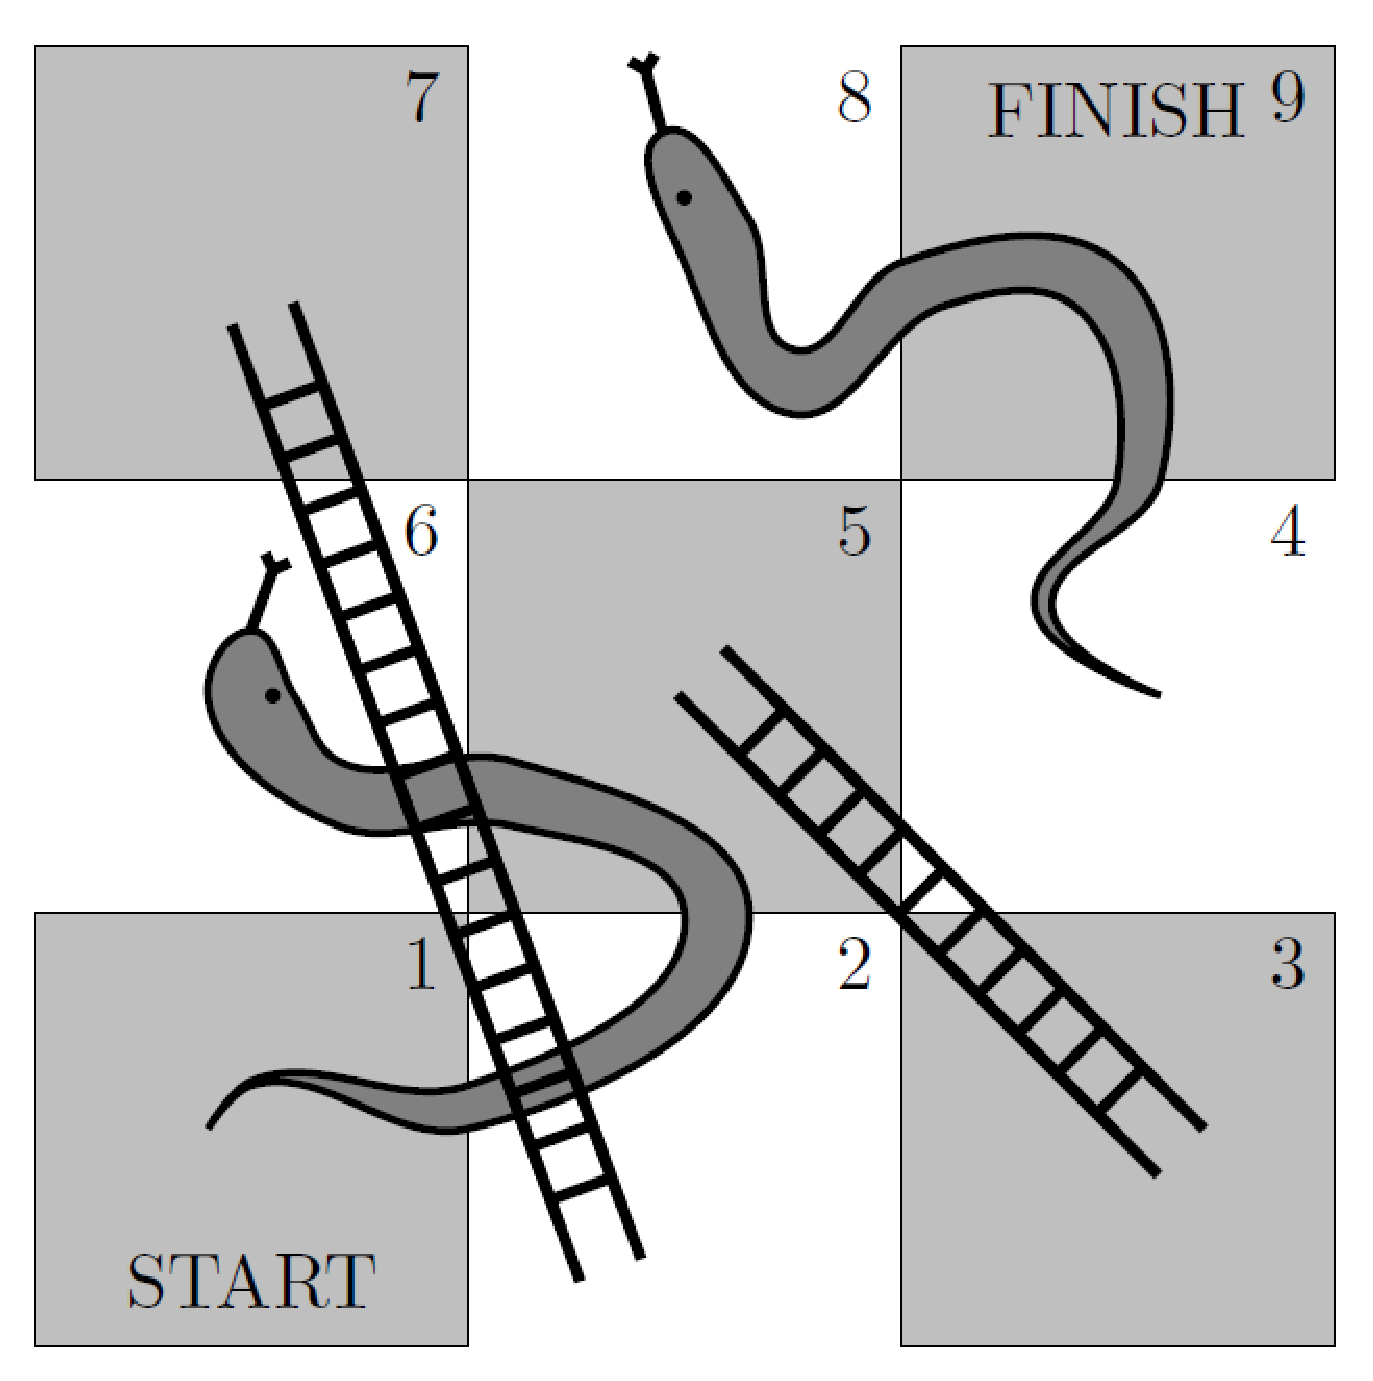
\includegraphics{Markov_chains/Markov_chains_1_1.eps}}
\end{figure}

At each turn a player tosses a fair coin and advances one or two places according to whether the coin lands heads or tails. If you land at the foot of a ladder you climb to the top, but if you land at the head of a snake you slide down to the tail. How many turn on average does it take to complete the game?

What is the probability that a player who has reached the middle square will complete the game without slipping back to square 1?
\end{exercise}

Solution. The transition matrix is
\be
\ba{c}
\ba{cccccc}
& \ 1 \ \ &\ 4 \ \ &\ 5\ \ &\ 7\ \ &\ 9\ \
\ea \\
\ba{c}
1 \\
4 \\
5 \\
7 \\
9
\ea
\lob
\ba{ccccc}
0 & 0 & \frac 12 & \frac 12 & 0 \\
\frac 12 & 0 & \frac 12 & 0 & 0 \\
\frac 12 & 0 & 0 & \frac 12 & 0  \\
0 & \frac 12 & 0 & 0 & \frac 12  \\
\ 0 \ \ & \ 0 \ \ & \ 0 \ \  &\  0 \ \  & \  1 \ \
\ea
\rob.
\ea
\ee

Let $k_i=\E_i(\text{time to hit 9})$ and $k_9=0$. We have
\be
\left\{\ba{l}
k_1 = 1 + \frac 12 k_7 + \frac 12 k_5\\
\\
k_4 = 1 + \frac 12 k_5 + \frac 12 k_1\\
\\
k_5 = 1 + \frac 12 k_1 + \frac 12 k_7\\
\\
k_7 = 1 + \frac 12 k_4 + \frac 12 k_9
\ea\right.\ \ra \
\left\{\ba{l}
k_1 = 1 + \frac 12 k_7 + \frac 12 k_5\\
\\
k_4 = 1 + \frac 12 k_5 + \frac 12 k_1\\
\\
k_5 = 1 + \frac 12 k_1 + \frac 12 k_7\\
\\
k_7 = 1 + \frac 12 k_4
\ea\right. \ \ra \
\left\{\ba{l}
k_1 = 7\\
\\
k_4 = 8\\
\\
k_5 = 7\\
\\
k_7 = 5
\ea\right.
\ee

Let $h_i=\pro_i(\text{hit 9 before 1})$ and $h_1=0, h_9=1$. We have
\be
\left\{\ba{l}
h_4 = \frac 12 h_5 + \frac 12 h_1\\
\\
h_5 = \frac 12 h_1 + \frac 12 h_7\\
\\
h_7 = \frac 12 h_4 + \frac 12 h_9
\ea\right.\ \ra \
\left\{\ba{l}
h_4 = \frac 12 h_5\\
\\
h_5 = \frac 12 h_7\\
\\
h_7 = \frac 12 h_4 + \frac 12
\ea\right. \ \ra \
\left\{\ba{l}
h_4 = \frac 17\\
\\
h_5 = \frac 27\\
\\
h_7 = \frac 47
\ea\right.
\ee

\begin{exercise}
Let $(X_n)_{n\geq 0}$ be a Markov chain on $\{0,1,\dots\}$ with transition probabilities given by
\be
p_{01}=1,\quad p_{ii+1}+p_{ii-1}=1, \quad p_{ii+1}=\lob\frac{i+1}{i}\rob^2p_{ii-1},\quad i\geq 1
\ee

Show that if $X_0=0$ the probability that $X_n\geq 1$ for all $n\geq 1$ is $6/\pi^2$.
\end{exercise}

Solution. Let $h_i=\pro_i(\text{hit 0})$ and $h_0=1$. We have
\be
h_{i} = p_{ii+1}h_{i+1} + p_{ii-1}h_{i-1}
\ee

so $u_{i} = h_{i-1}-h_i$ satisfies
\be
p_{ii+1}u_{i+1} = p_{ii-1}u_i \ \ra \ u_{i+1} = \lob \frac{p_{ii-1}}{p_{ii+1}}\rob u_i \ \ra \ u_{i+1} = \lob \frac{i}{i+1}\rob^2 u_i = \lob \frac{1}{i+1}\rob^2 u_1
\ee

Thus, we have
\be
h_i = h_0 - (h_0-h_i) = 1 - \sum^i_{k=1} u_k = 1-u_1\sum^i_{k=1}\frac 1{k^2}.
\ee

Since $(h_i:i\geq 0)$ is the minimal non-negative solution, $h_\infty=0$. so
\be
u_1=\lob\sum^\infty_{k=1}\frac 1{k^2}\rob^{-1} = \frac 6{\pi^2}\quad (\text{Basel problem})
\ee

Thus,
\be
\pro_0(X_n\geq 1,\ \forall n\geq 1) = 1- h_1 = \frac 6{\pi^2}.
\ee

\begin{exercise}
Let $(Y_n)_{n\geq 0}$ be independent identically distributed random with $\pro(Y_j=1)=\pro(Y_j=-1)=1/2$. Set $X_0=1$ and $X_n=X_0+Y_1+\dots+Y_n,\ n\geq 1$. Define the extinction time $H_0$ (the time of hitting 0) and find the probability generating function $\phi(s)=\E_1s^{H_0}$. Calculate the mean value $\E_1H_0$.

Suppose the distribution of $Y_j$ is changed to $\pro(Y_j=2)=\pro(Y_j=-1)=1/2$. Show that $\phi$ now satisfies
\be
s\phi^3-2\phi +s =0.
\ee
\end{exercise}

Solution. We know that the probability generating function of a sum of independent random variables is simply the product of the probability generating functions. Thus,
\be
\phi(s) = \E_1s^{H_0} = \frac 12\E_2s^{H_0+1} +\frac 12\E_0s^{H_0+1} = \frac s2\E_2s^{H_0}+\frac{s}{2}\E_0s^{H_0} = \frac s2 \phi^2(s) + \frac s2
\ee

So we have
\be
s\phi^2 - 2\phi + s = 0 \ \ra \ \phi(s) = \frac {2\pm\sqrt{4-4s^2}}{2s} = \frac {1\pm\sqrt{1-s^2}}s
\ee

Since $\phi(0)=0$, we choose
\be
\phi(s) = \frac {1-\sqrt{1-s^2}}s \ \ra \ \phi'(s) = \frac{s(-1/2)(-2s)(1-s^2)^{-1/2}- (1-\sqrt{1-s^2})}{s^2} = \frac {1-\sqrt{1-s^2}}{s^2\sqrt{1-s^2}}
\ee

Thus,
\be
\E_1H_0 = \lim_{s\to 1^-}\phi'(s) = \infty.
\ee

If $\pro(Y_j=2)=\pro(Y_j=-1)=1/2$, we have
\be
\phi(s) = \frac s2\E_3s^{H_0}+\frac s2\E_0s^{H_0} = \frac s2 \phi^3(s)+ \frac s2 \ \ra \ s\phi^3-2\phi +s =0
\ee
as required.

\begin{exercise}
A random sequence of non-negative integers $(F_n)_{n\geq 0}$ is obtained by setting $F_0=0$ and $F_1=1$ and, one $F_0,\dots,F_n$ are known, taking $F_{n+1}$ to be either the sum or the difference of $F_{n-1}$ and $F_n$, each with probability $1/2$. Is $(F_n)_{n\geq 0}$ a Markov chain? By considering the Markov chain $X_n=(F_{n-1},F_n)$, find the probability that $(F_n)_{n\geq 0}$ reaches 3 before first returning to 0.

Draw enough of the flow diagram for $(F_n)_{n\geq 0}$ to establish a general pattern. Hence, using the strong Markov property, show that the hitting probability for $(1,1)$, starting from $(1,2)$, is $(3-\sqrt{5})/2$. Deduce that $F_n\to \infty$ as $n\to \infty$.
\end{exercise}

Solution. $(F_n)$ is not a Markov chain, as $F_{n+1}$ depends on $F_n$ and $F_{n-1}$, but the pair $(F_{n-1},F_n)$ is.

\centertexdraw{

    \def\bdot {\fcir f:0 r:0.025 }

    \drawdim in

    \arrowheadtype t:F \arrowheadsize l:0.08 w:0.04
    \linewd 0.01 \setgray 0

    \move (1 0)\bdot
    \move (0 0)\bdot
    \move (0.5 0.5)\bdot
    \move (0.2 1)\bdot
    \move (0.8 1)\bdot
    \move (0 -0.5)\bdot
    \move (-0.3 -0.5)\bdot
    \move (0.3 -1)\bdot
    \move (0.0 -1)\bdot
    \move (-0.3 -1)\bdot
    \move (-0.6 -1)\bdot
    \move (1 -0.5)\bdot
    \move (1.3 -0.5)\bdot
    \move (1.3 -1)\bdot
    \move (1.6 -1)\bdot
    \move (1 -1)\bdot
    \move (0.7 -1)\bdot

    \move (0.9 0) \avec(0.5 0) \move(0.9 0) \lvec (0.1 0)
    \move (0.05 0.05) \avec(0.25 0.25) \move(0.05 0.05) \lvec (0.45 0.45)
    \move (0.55 0.45) \avec(0.75 0.25) \move(0.55 0.45) \lvec (0.95 0.05)
    \move (0.45 0.55) \avec(0.35 0.75) \move(0.45 0.55) \lvec (0.25 0.95)
    \move (0.25 1) \avec(0.5 1) \move(0.25 1) \lvec (0.75 1)
    \move (0.75 0.95) \avec(0.65 0.75) \move(0.75 0.95) \lvec (0.55 0.55)

    \move (0 -0.05) \avec(0 -0.25) \move(0 -0.05) \lvec (0 -0.45)
    \move (-0.05 -0.5) \avec(-0.2 -0.5) \move(-0.05 -0.5) \lvec (-0.25 -0.5)
    \move (-0.25 -0.45) \avec(-0.1 -0.15) \move(-0.25 -0.45) \lvec (-0.05 -0.05)

    \move (1.05 -0.05) \avec(1.15 -0.25) \move(1.05 -0.05) \lvec (1.25 -0.45)
    \move (1.25 -0.5) \avec(1.1 -0.5) \move(1.25 -0.5) \lvec (1.05 -0.5)
    \move (1 -0.45) \avec(1 -0.25) \move(1 -0.45) \lvec (1 -0.05)

    \move (-0.3 -0.55) \avec(-0.3 -0.75) \move(-0.3 -0.55) \lvec (-0.3 -0.95)
    \move (-0.35 -1) \avec(-0.5 -1) \move(-0.35 -1) \lvec (-0.55 -1)
    \move (-0.55 -0.95) \avec(-0.4 -0.65) \move(-0.55 -0.95) \lvec (-0.35 -0.55)

    \move (0.05 -0.55) \avec(0.15 -0.75) \move(0.05 -0.55) \lvec (0.25 -0.95)
    \move (0.25 -1) \avec(0.1 -1) \move(0.25 -1) \lvec (0.05 -1)
    \move (0 -0.95) \avec(0 -0.75) \move(0 -0.95) \lvec (0 -0.55)

    \move (1 -0.55) \avec(1 -0.75) \move(1 -0.55) \lvec (1 -0.95)
    \move (0.95 -1) \avec(0.8 -1) \move(0.95 -1) \lvec (0.75 -1)
    \move (0.75 -0.95) \avec(0.9 -0.65) \move(0.75 -0.95) \lvec (0.95 -0.55)

    \move (1.35 -0.55) \avec(1.45 -0.75) \move(1.35 -0.55) \lvec (1.55 -0.95)
    \move (1.55 -1) \avec(1.4 -1) \move(1.55 -1) \lvec (1.35 -1)
    \move (1.3 -0.95) \avec(1.3 -0.75) \move(1.3 -0.95) \lvec (1.3 -0.55)

    \htext (-0.35 -0.05){(2,1)}
    \htext (1.05 -0.05){(1,2)}
    \htext (0.1 0.45){(1,1)}
    \htext (-0.15 0.95){(1,0)}
    \htext (0.85 0.95){(0,1)}

    \htext (0.65 -0.55){(3,1)}
    \htext (1.35 -0.55){(2,3)}

    \htext (-0.65 -0.55){(3,2)}
    \htext (0.05 -0.55){(1,3)}

    \htext (-0.95 -1.05){(5,3)}
    \htext (1.65 -1.05){(3,5)}

    \htext (-0.5 -1.2){(2,5)}
    \htext (-0.15 -1.2){(4,1)}
    \htext (0.2 -1.2){(3,4)}

    \htext (0.55 -1.2){(4,3)}
    \htext (0.9 -1.2){(1,4)}
    \htext (1.25 -1.2){(5,2)}

\move (0 1.2)
\move (0 -1.3)
}

The initial part of the diagram shows that the level $F_n=3$ can be reached from $(F_0,F_1)=(0,1)$ either at (2,3) or (1,3). To hit this level before visiting level $F_n=0$ (i.e. (1,0)), we have two straight paths, supplemented with a number of adjacent triangular cycles. The two possibilities give the probability
\be
1\cdot \frac 12 \cdot \frac 12 \lob 1+ \frac 18 + \frac 1{8^2} + \cdots\rob = \frac 27,\quad 1\cdot \frac 12 \cdot \frac 12 \cdot \frac 12 \lob 1+ \frac 18 + \frac 1{8^2} + \cdots\rob = \frac 17,
\ee
which adds to 3/7.

One can see a triangular 'pattern' emerging from the diagram, with treelike symmetries. In particular, we define
\be
\left\{\ba{l}
p:=\pro_{(1,2)}(\text{hit (1,1)}) = \pro_{(2,3)}(\text{hit (1,2)}) = \pro_{(1,3)}(\text{hit (2,1)})\\
\\
p':=  \pro_{(2,1)}(\text{hit (1,1)}) = \pro_{(3,2)}(\text{hit (2,1)}) = \pro_{(3,1)}(\text{hit (1,2)})
\ea\right.
\ee

Conditioning on the first jump, by the strong Markov property, we can write
\be
\left\{\ba{l}
\pro_{(1,2)}(\text{hit (1,1)}) = \frac 12 \pro_{(2,3)}(\text{hit (1,1)}) + \frac 12 \pro_{(2,1)}(\text{hit (1,1)}) \\
\\
\pro_{(2,1)}(\text{hit (1,1)}) = \frac 12 \pro_{(1,3)}(\text{hit (1,1)}) + \frac 12
\ea\right.\ \ra \
\left\{\ba{l}
p = \frac 12 p^2 + \frac 12 p'\\
\\
p' = \frac 12 pp' + \frac 12
\ea\right.
\ee

Then we have
\be
(p-1)(p^2-3p+1)=0\ \ra \ p=1,(3\pm\sqrt{5})/2.
\ee

We are interested in the minimal non-negative root. Thus the probability should be $(3-\sqrt{5})/2$.

We know (1,1) is transient (because $p<1$), so the (only) communicating class is transient. Thus, we have
\be
\pro(X_n=(i,j) \text{ for infinitely many }n) = 0,\ \forall (i,j) \ \ra \ \pro(F_n=i \text{ for infinitely many }n) = 0,\ \forall i
\ee

Suppose that $F_n\nrightarrow\infty$ as $n\to \infty$. Thus $\exists K:\forall N\in\N$, $\exists n\geq N$ s.t. $F_n\leq K$ for infinitely many $n$. Thus, $\exists i\leq K: F_n=j$ for infinitely many $n$ and
\be
\pro(F_n=i \text{ for infinitely many }n) = 0\ \ra \ \pro(F_n\nrightarrow \infty) = 0 \ \ra \ \pro(F_n\to \infty) = 1.
\ee

Now we consider more general case: taking the sum with $q$ and taking the difference with $1-q$. Thus, we have
\be
\left\{\ba{l}
\pro_{(1,2)}(\text{hit (1,1)}) = q \pro_{(2,3)}(\text{hit (1,1)}) + (1-q) \pro_{(2,1)}(\text{hit (1,1)}) \\
\\
\pro_{(2,1)}(\text{hit (1,1)}) = q \pro_{(1,3)}(\text{hit (1,1)}) + 1-q
\ea\right.\ \ra \
\left\{\ba{l}
p = q p^2 + (1-q) p'\\
\\
p' = q pp' + (1-q)
\ea\right.
\ee
Then we have (if $0<q\leq 1$)
\be
(p-1)(q^2p^2-q(2-q)p+(1-q)^2)=0\ \ra \ p=1,\frac {2-q\pm\sqrt{4q-3q^2}}{2q}.
\ee

We see that $\frac {2-q-\sqrt{4q-3q^2}}{2q}>0$ and we take it as the minimal non-negative root if
\be
\frac {2-q -\sqrt{4q-3q^2}}{2q}<1 \ \ra \ q>\frac 13
\ee
otherwise, we take 1 as the minimal non-negative root. In other case $q=0$, it is easy to see that $p=1$. Thus,
\be
\left\{\ba{cl}
\frac {2-q-\sqrt{4q-3q^2}}{2q} \quad\quad & q>\frac 13\\
\\
1 & q \leq \frac 13
\ea\right.
\ee

\vspace{2mm}

%%%%%%%%%%%%%%%%%%%%%%%%%%%%%%%%%

\begin{exercise}
The rooted binary tree is an infinite graph $T$ with one distinguished vertex $R$ from which comes a single edge; at every other vertex there are three edges and there are no closed loops. The random walk on $T$ jumps from a vertex along each available edge with equal probability. Show that the random walk is transient.
\end{exercise}

Solution. Let $(X_n)_{n\geq 0}$ be the distance (the length of the shortest path) from $R$. Then $(X_n)_{n\geq 0}$ is a Markov chain on $\N_0$ with transition probabilities $p_{i,i+1} = \frac 23$ and $p_{i,i+1} = \frac 13$.

Let $h_i = \pro_i(\text{hit } 0)$. We have the recurrence relation
\be
h_i = \frac 13 h_{i-1} + \frac 23 h_{i+1}
\ee
for $i \geq 1$ with boundary condition $h_0 = 1$. The minimal non-negative solution to this recurrence relation is $h_i = \bb{\frac 12 }^i$. Since $h_1 = \pro_R(\text{return to }R) < 1$, the random walk is transient.

\begin{exercise}
Let $(X_n)_{n\geq 0}$ be a Markov chain on $\{0,1,\dots\}$ with transition probabilities given by
\be
p_{01}=1,\quad p_{ii+1}+p_{ii-1}=1, \quad p_{ii+1}=\lob\frac{i+1}{i}\rob^\alpha p_{ii-1},\quad i\geq 1,\ \alpha \in(0,\infty)
\ee

What is the value of $\pro(X_n\to\infty\text{ as }n\to\infty)$?
\end{exercise}

Solution. Let $h_i=\pro_i(\text{hit 0})$ and $h_0=1$. We have
\be
h_{i} = p_{ii+1}h_{i+1} + p_{ii-1}h_{i-1}
\ee

so $u_{i} = h_{i-1}-h_i$ satisfies
\be
p_{ii+1}u_{i+1} = p_{ii-1}u_i \ \ra \ u_{i+1} = \lob \frac{p_{ii-1}}{p_{ii+1}}\rob u_i \ \ra \ u_{i+1} = \lob \frac{i}{i+1}\rob^\alpha u_i = \lob \frac{1}{i+1}\rob^\alpha u_1
\ee

Thus, we have
\be
h_i = h_0 - (h_0-h_i) = 1 - \sum^i_{k=1} u_k = 1-u_1\sum^i_{k=1}\frac 1{k^\alpha}.
\ee

Since $(h_i:i\geq 0)$ is the minimal non-negative solution, $h_\infty=0$. so
\be
u_1=\lob\sum^\infty_{k=1}\frac 1{k^\alpha}\rob^{-1} \ \ra \ h_i = 1-\left.\sum^i_{k=1}\frac 1{k^\alpha}\right/\sum^\infty_{k=1}\frac 1{k^\alpha}.
\ee

Thus,
\be
h_i=\left\{\ba{ll}
=1 \quad\quad & \text{if } \sum^\infty_{k=1}\frac 1{k^\alpha} =\infty \ (\alpha\leq 1)\\
\\
<1 & \text{if } \sum^\infty_{k=1}\frac 1{k^\alpha} < \infty \ (\alpha >  1)
\ea\right.\ \ra \
(X_n)_{n\geq 0} \text{ is }\left\{
\ba{l}
\text{recurrent if }\alpha\leq 1\\
\text{transient if }\alpha > 1
\ea\right.
\ee

Equivalently,
\be
\pro(X_n\to\infty\text{ as }n\to\infty)
=\left\{\ba{ll}
0 \quad\quad & \text{if } \alpha\leq 1\\
1 & \text{if } \alpha >  1
\ea\right.
\ee

\begin{exercise}
Show that the simple symmetric random walk in $\Z^4$ is transient.
\end{exercise}

Solution. We project the random walk $(X_n^d)$ on $\Z^d$ to three dimensions by discarding all coordinates but the first three. The project chain $(X_n^{\text{proj}})$ on $\Z^3$ stays where it is with probability $(d-3)/d$, but when it jumps, it behaves as the nearest-neighbour symmetric walk in dimension 3.

Let $(X_n)_{n\geq 0}$ be the simple symmetric random walk in $\Z^4$ with
\be
p_{ij}=\left\{
\ba{ll}
1/8 \quad \quad &\text{if }|i-j|=1\\
0 & \text{otherwise}
\ea
\right.\quad\quad i,j\in\Z^4
\ee

Let $(Y_m)_{m\geq 0}$ be the projection of $(X_n)_{n\geq 0}$ on $\Z^3$ with
\be
\tilde{p}_{ij}=\left\{
\ba{ll}
1/4  & \text{if }|i-j|=0 \\
1/8 \quad \quad &\text{if }|i-j|=1\\
0 & \text{otherwise}
\ea
\right. \quad\quad i,j\in\Z^3
\ee

Observe $(Y_{m})_{m\geq 0}$ only when it moves, the resulting process $(Z_t)_{t\geq 0}$ is given by $Z_t=Y_{S_t}$ where $S_0=0$ and
\be
S_{t+1} = \inf\{m\geq S_t: Y_m \neq Y_{S_t}\}
\ee
so $S_t$ is a stopping time and by strong Markov property
\beast
& & \pro(Z_{t+1}=i_{t+1}|Z_0=i_0,\dots,Z_t=i_t) \\
& = & \pro(Y_{S_{t+1}}=i_{t+1}|Y_{S_0}=i_0,\dots,Y_{S_t}=i_t) = \pro_{i_t}(Y_{S_1}=i_{t+1}) \quad (\text{since $Y$ is Markov chain})\\
& = & \hat{p}_{i_ti_{t+1}}
\eeast
so $Z$ is Markov chain with transition matrix $\hat{P}$ where $\hat{p}_{ii}=0$ and for $i\neq j$
\be
\hat{p}_{ij} = \frac{\tilde{p}_{ij}}{\sum_{k\neq i}\tilde{p}_{ik}}
\ee
so we have
\be
p_{ij}=\left\{
\ba{ll}
1/6 \quad \quad &\text{if }|i-j|=1\\
0 & \text{otherwise}
\ea
\right.\quad\quad i,j\in\Z^4
\ee
thus $(Z_t)_{t\geq 0}$ is the simple symmetric random walk in $\Z^3$. We know $(Z_t)_{t\geq 0}$ is transient, so $\sum_{n\geq 0}\hat{p}_{ii}^{(n)}<\infty$. Also, we have $p_ii^{(n)}< \tilde{p}_ii^{(n)}<\hat{p}_ii^{(n)}$. Hence,
\be
\sum_{n\geq 0}p_{ii}^{(n)}< \sum_{n\geq 0}\tilde{p}_{ii}^{(n)}<\sum_{n\geq 0}\hat{p}_{ii}^{(n)}<\infty
\ee

\begin{exercise}
Find all invariant distributions of the transition matrix
\be
P=
\lob
\ba{ccccc}
\frac 12 & 0 & 0 & 0 & \frac 12 \\
0 & \frac 12 & 0 & \frac 12 & 0 \\
0 & 0 &  1 & 0 & 0  \\
0 & \frac 14 &  \frac 14 & \frac 14 & \frac 14  \\
\ \frac 12 \ \  & \ 0 \ \ & \ 0 \ \  &\  0 \ \  &  \ \frac 12 \ \
\ea
\rob.
\ee
\end{exercise}

Solution. We have
\be
\pi P = \pi \ \ra \ \pi = \lob\frac 12 p,0,1-p,0,\frac 12 p\rob,\quad 0\leq p\leq 1
\ee

This is not unique. This example shows that the non-uniqueness occurs when the matrix is not irreducible.

\begin{exercise}
Gas molecules move about randomly in a box which is divided into two halves symmetrically by a partition. A hole is made in the partition. Suppose there are $N$ molecules in the box. Show that the number of molecules on the side of the partition just after a molecule has passed through the hole evolves as a Markov chain. What are the transition probabilities? What is the invariant distribution of this chain?
\end{exercise}

Solution. The state-space is \{0,1,\dots,N\} and the transition probabilities are
\be
p_{i,i+1} + p_{i,i-1} = 1, \quad p_{i,i-1} = \frac iN,\ i=1,\dots,N
\ee

Since the Markov chain is reversible, $P$ and $\pi$ are in detailed balance, i.e.
\be
\pi_ip_{i,i-1} = \pi_{i-1}p_{i-1,i} \ \ra \ \pi_i = \frac{p_{i-1,i}}{p_{i,i-1}}\pi_{i-1} = \frac{1-\frac {i-1}N}{\frac iN}\pi_{i-1} =\frac{N-i+1}{i}\pi_{i-1} = \binom{N}{i}\pi_0
\ee

Then we have
\be
1 = \sum^N_{i=0}\pi_i = \sum^N_{i=1}\binom{N}{i}\pi_0 = \pi_02^N \ \ra \ \pi_0=\lob\frac 12\rob^N \ \ra \ \pi_i = \binom{N}{i}\lob\frac 12\rob^N \ \ra \ \pi_i \sim \text{Bin}\lob N,\frac 12\rob.
\ee

\begin{exercise}
A particle moves on the eight vertices of a cube in the following way: at each step the particle is equally likely to move to each of the three adjacent vertices, independently of its past motion. Let $i$ be the initial vertex occupied by the particle, $o$ the vertex opposite $i$. Calculate each of the following quantities:

(i) the expected number of steps until the particle returns to $i$;

(ii) the expected number of visits to $o$ until the first return to $i$;

(iii) the expected number of steps until the first visit to $o$.
\end{exercise}

Solution. Draw the diagram

\centertexdraw{

    \def\bdot {\fcir f:0 r:0.025 }

    \drawdim in

    \arrowheadtype t:F \arrowheadsize l:0.08 w:0.04
    \linewd 0.01 \setgray 0

    \move (0 0)\bdot
    \move (1 0)\bdot
    \move (0 1)\bdot
    \move (1 1)\bdot
    \move (0.5 0.3)\bdot
    \move (1.5 0.3)\bdot
    \move (0.5 1.3)\bdot
    \move (1.5 1.3)\bdot

    \move (0 0) \lvec (1 0) \lvec(1 1) \lvec(0 1) \lvec(0 0)
    \move (0 1) \lvec(0.5 1.3) \lvec(1.5 1.3) \lvec(1 1)
    \move (1 0) \lvec(1.5 0.3) \lvec(1.5 1.3)

    \linewd 0.01 \lpatt(0.067 0.1)

    \move (0 0) \lvec (0.5 0.3) \lvec (0.5 1.3) \move(0.5 0.3) \lvec(1.5 0.3)

    \htext (-0.1 1.05){1}
    \htext (0.9 1.05){2}
    \htext (-0.1 -0.15){3}
    \htext (0.9 -0.15){4}

    \htext (0.4 1.35){5}
    \htext (1.4 1.35){6}
    \htext (0.35 0.3){7}
    \htext (1.55 0.25){8}
}

We take 1 as $i$ and 8 as $o$ and the transition probabilities are given by
\be
p_{ij}=\left\{
\ba{ll}
1/3 \quad \quad &\text{if $i$ and $j$ are connected}\\
0 & \text{otherwise}
\ea
\right.\quad\quad
\ee

Thus the equilibrium distribution is $\pi = (\frac 18, \frac 18,\frac 18,\frac 18,\frac 18,\frac 18,\frac 18,\frac 18)$.

(i) Since the Markov chain is irreducible and positive recurrent, we have
\be
m_k = \E_kT_k = \frac 1{\pi_k}\ \ra \ m_1 = \frac 1{\pi_1} = 8.
\ee

(ii) With the same condition, we have $\forall j\neq k$
\be
\E_k(\text{number of visits to $j$ before returning to $k$}) = \frac {\pi_j}{\pi_k} = 1.
\ee

(iii) We see that 2, 3, 5 are symmetric as well as 4, 6, 7. Thus we have 4-state Markov chain \{I(1), II(2,3,5), III(4,6,7), IV(8)\} and let $k_i=\E_i(\text{time to hit 8})$. We have $k_{IV}=0$ and
\be
\left\{
\ba{l}
k_I = 1 + k_{II} \\
\\
k_{II} = 1 + \frac 13k_I + \frac 23 k_{III}\\
\\
k_{III} = 1 + \frac 13k_{IV} + \frac 23k_{II}
\ea\right. \ \ra \
k_I = 10,\ k_{II} = 9, \ k_{III} = 7.
\ee

Thus, the answer is 10.

\begin{exercise}
Let $(X_n)_{n\geq 0}$ be a Markov chain on $\{1,2,3\}$ with transition matrix
\be
\lob
\ba{ccc}
0 & 1 & 0 \\
0 & \frac 23 & \frac 13 \\
p &  \quad 1-p\quad \quad & 0
\ea
\rob.
\ee

Find the invariant distributions of the transition matries when (a) $p=\frac{1}{16}$,  (b)  $p=\frac{1}{6}$, (c)  $p=\frac{1}{12}$. (in Example Sheet 1)
\end{exercise}

Solution. With the definition of invariant distribution, we have
\be
\pi
\lob
\ba{ccc}
0 & 1 & 0 \\
0 & \frac 23 & \frac 13 \\
p &  \quad 1-p\quad \quad & 0
\ea
\rob = \pi \ \ra \ \pi = \frac 1{p+4}(p,3,1) \ \ra \ \pi_1=\lim_{n\to\infty}\pro(X_n=1|X_0=1)=\frac p{p+4}.
\ee

Check the results in Example 1 we have

(a) $p=\frac 1{16}\ \ra \ \pi_1 = \frac{1/16}{1/16+4} = \frac 1{65} = \lim_{n\to\infty}p_{11}^{(n)} = \lim_{n\to\infty}\frac 1{65} -\frac 25\lob-\frac 14\rob^n + \frac {18}{13} \lob -\frac{1}{12}\rob^n$.

(b) $p=\frac 1{6}\ \ra \ \pi_1 = \frac{1/6}{1/6+4} = \frac 1{25} = \lim_{n\to\infty}p_{11}^{(n)} = \lim_{n\to\infty}\frac 1{25} + \lob \frac 1{3\sqrt{2}}\rob^n \lob \frac {24}{25}\cos\frac{3n\pi}4 +\frac {18}{25}\sin\frac{3n\pi}4\rob$.

(c) $p=\frac 1{12}\ \ra \ \pi_1 = \frac{1/12}{1/12+4} = \frac 1{49} = \lim_{n\to\infty}p_{11}^{(n)} = \lim_{n\to\infty}\frac 1{49} + \lob\frac {48}{49}-\frac {6}{7}n\rob\lob-\frac 1{6}\rob^n$.

\begin{exercise}
A fair die is thrown repeatedly. Let $X_n$ denote the sum of the first $n$ throws. Find
\be
\lim_{n\to\infty}\pro(X_n\text{ is a multiple of 13}).
\ee
\end{exercise}

Solution. Let $(X_n)_{n\geq 0}$ denote the sum of the first $n$ throws and $Y_n=X_n\bmod 13$. Thus, the its transition probabilities are given by
\be
p_{ij} = 1/6, \quad \text{for }j=(i+k)\bmod 13, \ k=1,2,3,4,5,6
\ee

Obviously, $P$ is irreducible. Also, we have $p_{00}^{(2)}>0$, $p_{00}^{(3)}>0$ and gcd(2,3)=1. Thus, we can see that state 0 is aperiodic (with the conclusion that state $i$ is aperiodic if and only if the set $\{n\geq 0:p_{ii}^{(n)}>0\}$ has no common divisor other than 1). So the irreducibility and aperiodicity imply that
\be
p_{ij}^{(n)}\to \pi_j,\quad \quad \text{as }n\to \infty
\ee

By symmetry, $\pi_i=1/13,\ \forall i$. Hence,
\be
\lim_{n\to\infty}\pro(X_n\text{ is a multiple of 13}) = \lim_{n\to\infty}\pro(Y_n=0) = \lim_{n\to\infty}p_{i0} = \pi_0 = \frac 1{13}.
\ee

\begin{exercise}
Each morning a student takes one of the three books she owns from her shelf. The probability that she chooses book $i$ is $\alpha_i$, $0<\alpha_i<1,\ i=1,2,3$, and choices on successive days are independent. In the evening she replaces the book at the left-hand end of the shelf. If $p_n$ denotes the probability that on day $n$ the student finds the books in the order 1,2,3, from left to right, show that, irrespective of the initial arrangement of the books, $p_n$ converges as $n\to \infty$, and determine the limit.
\end{exercise}

Solution. First we draw the diagram and Set 6-state Markov chain 1(123), 2(132), 3(213), 4(231), 5(312), 6(321).

\centertexdraw{

%\def\bdot {\fcir f:0 r:0.025 }

\drawdim in
\arrowheadtype t:F \arrowheadsize l:0.08 w:0.04
\linewd 0.01 \setgray 0

\move (0 0)\lcir r:0.15
\htext (-0.1 -0.05) {123}
\move (1 0)\lcir r:0.15
\htext (0.9 -0.05) {231}
\move (2 0)\lcir r:0.15
\htext (1.9 -0.05) {312}

\move (0 -0.8)\lcir r:0.15
\htext (-0.1 -0.85) {213}
\move (1 -0.8)\lcir r:0.15
\htext (0.9 -0.85) {321}
\move (2 -0.8)\lcir r:0.15
\htext (1.9 -0.85) {132}

\move (-0.05 -0.2) \avec(-0.05 -0.6)
\move (0.05 -0.6) \avec(0.05 -0.2)
\move (0.95 -0.2) \avec(0.95 -0.6)
\move (1.05 -0.6) \avec(1.05 -0.2)
\move (1.95 -0.2) \avec(1.95 -0.6)
\move (2.05 -0.6) \avec(2.05 -0.2)

\move (0.8 0) \avec(0.2 0)
\move (1.8 0) \avec(1.2 0)

\move (0.2 -0.8) \avec(0.8 -0.8)
\move (1.2 -0.8) \avec(1.8 -0.8)

\move (-0.15 0.15) \larc r:0.1 sd:0 ed:270
\move (-0.215 0.225) \avec(-0.225 0.215)
\move (1 0.2) \larc r:0.1 sd:-45 ed:225
\move (1.005 0.3) \avec(0.995 0.3)
\move (2.15 0.15) \larc r:0.1 sd:-90 ed:180
\move (2.225 0.215) \avec(2.215 0.225)

\move (-0.15 -0.95) \larc r:0.1 sd:90 ed:360
\move (-0.215 -1.025) \avec(-0.225 -1.015)
\move (1 -1) \larc r:0.1 sd:135 ed:45
\move (1.005 -1.1) \avec(0.995 -1.1)
\move (2.15 -0.95) \larc r:0.1 sd:180 ed:450
\move (2.225 -1.015) \avec(2.215 -1.025)

\move (1 -1) \larc r:1.45 sd:55 ed:125
\move (0.995 0.45) \avec(1.005 0.45)

\move (1 0.2) \larc r:1.45 sd:235 ed:305
\move (1.005 -1.25) \avec(0.995 -1.25)

\htext (-0.25 -0.4){$\alpha_2$}
\htext (0.1 -0.4){$\alpha_1$}
\htext (0.75 -0.4){$\alpha_3$}
\htext (1.1 -0.4){$\alpha_2$}
\htext (1.75 -0.4){$\alpha_1$}
\htext (2.1 -0.4){$\alpha_3$}

\htext (0.5 0.05){$\alpha_1$}
\htext (1.5 0.05){$\alpha_2$}
\htext (0.5 -0.95){$\alpha_3$}
\htext (1.5 -0.95){$\alpha_1$}

\htext (-0.4 0.1){$\alpha_1$}
\htext (1.15 0.2){$\alpha_2$}
\htext (2.3 0.1){$\alpha_3$}
\htext (-0.4 -0.9){$\alpha_2$}
\htext (1.15 -1){$\alpha_3$}
\htext (2.3 -0.9){$\alpha_1$}

\htext (1 0.5){$\alpha_3$}
\htext (1 -1.4){$\alpha_2$}

\htext (3 -0.6){$P=\lob\ba{cccccc}
\alpha_1 & 0 & \alpha_2 & 0 & \alpha_3 & 0 \\
0 & \alpha_1 & \alpha_2 & 0 & \alpha_3 & 0 \\
\alpha_1 & 0 & \alpha_2 & 0 & 0 & \alpha_3 \\
\alpha_1 & 0 & 0 & \alpha_2 & 0 & \alpha_3 \\
0 & \alpha_1 & 0 & \alpha_2 & \alpha_3 & 0 \\
\ 0\ \ & \ \alpha_1 \ \ &\ 0\ \ &\ \alpha_2\ \ &\ 0\ \ &\ \alpha_3\ \ \\
\ea\rob$}

\move (6 0)
\move (6 0.8)
}

Obviously, the Markov chain is irreducible. It is also aperiodic since
\be
\left\{
\ba{ll}
123\to 312\to 231 \to 123&\text{3 steps} \\
123\to 213\to 321 \to 231 \to 123 \quad\quad &\text{4 steps}
\ea\right.\
\ee

Therefore, $p_n=p_{i1}\to \pi_1,\ \forall i$. With the definition of invariant distribution. we see that
\be
\left\{
\ba{l}
\pi_1 = \alpha_1(\pi_1+\pi_3+\pi_4) \\
\pi_2 = \alpha_1(\pi_2+\pi_5+\pi_6)
\ea\right.\ \ra \
\pi_1+\pi_2 =\alpha_1.
\ee

Similarly, we have $\pi_3+\pi_4 = \alpha_2$ and substitute it into $\pi_1 = \alpha_1(\pi_1+\pi_3+\pi_4)$
\be
\pi_1 = \alpha_1(\pi_1+\alpha_2) \ \ra \ \pi_1 = \frac {\alpha_1\alpha_2}{1-\alpha_1}.
\ee

\begin{exercise}
In each of the following cases determine whether the stochastic matrix $P$ is reversible:
\begin{align*}
& (a)\quad \lob
\ba{cc}
p & 1-p\\
q & \ 1-q \ \
\ea\rob
;\quad\quad\quad\quad
(b)\quad \lob
\ba{ccc}
0 & p & 1-p\\
1-p & 0 & p \\
p& 1-p & 0
\ea\rob;\\
& (c)\quad I=\{0,1,\dots, N\} \text{ and } p_{ij}=0\text{ if }|j-i|\geq 2; \\
& (d)\quad I=\{0,1,\dots, N\} \text{ and } p_{01} = 1,\ p_{ii+1}=p,\ p_{ii-1}=1-p \text{ for }i\geq 1. \quad\quad\quad\quad\quad\quad\quad\quad\quad\quad\quad\quad\quad\quad\quad\quad\quad\quad
\end{align*}
\end{exercise}

Solution. If there exists $\pi$ s.t.
\be
\pi_ip_{ij} = \pi_jp_{ji},\quad \forall i,j\in I
\ee
then $P$ is reversible.

(a) We have
\be
\pi_1p_{12} = \pi_2p_{21}\ \ra\ \pi_1(1-p)=\pi_2q \ \ra \ \pi_1=\frac q{1-p+q},\ \pi_2=\frac{1-p}{1-p+q}\ \ra \ P \text{ is reversible}.
\ee

(b)
\be
\left\{
\ba{l}
\pi_1p_{12} = \pi_2p_{21}\\
\pi_1p_{13} = \pi_3p_{31}\\
\pi_2p_{23} = \pi_3p_{32}
\ea\right.\ \ra \
\left\{
\ba{l}
\pi_2 = \frac{p^2}{(1-p)^2}\pi_3\\
\pi_2 = \frac{1-p}p\pi_3
\ea\right.\ \ra \ p^3 = (1-p)^3 \ \ra \ p=\frac 12 \ \ra \ P \text{ is reversible iff }p=\frac 12.
\ee

(c)
\be
\left\{\ba{l}
\pi_ip_{i,i+1} = \pi_{i+1}p_{i+1,i} \\
\quad \quad \ \ra \ \pi_{i+1}=\frac{p_{i,i+1}}{p_{i+1,i}}\pi_i = \lob\prod^i_{k=0}\frac{p_{k,k+1}}{p_{k+1,k}}\rob\pi_0 \\
\sum^N_{i=0}\pi_i=1
\ea \right.\ \ra \
\pi_i = \frac{\prod^{i-1}_{k=0}\frac{p_{k,k+1}}{p_{k+1,k}}}{1+\sum^N_{i=1}\lob\prod^{i-1}_{k=0}\frac{p_{k,k+1}}{p_{k+1,k}}\rob} \ \ra \ P \text{ is reversible}.
\ee

(d)
\be
\left\{\ba{l}
\pi_0p_{01} = \pi_1p_{10} \ \ra \ \pi_0=(1-p)\pi_1\\
\pi_ip_{i,i+1} = \pi_{i+1}p_{i+1,i},\ i\geq 1\\
\quad \quad \ \ra \ \pi_{i+1}=\frac{p}{1-p}\pi_i = \frac 1p\lob\frac{p}{1-p}\rob^{i+1}\pi_0 \\
\sum^\infty_{i=0}\pi_i=1
\ea \right.\ \ra \
\pi_i = \frac{\lob\frac{p}{1-p}\rob^{i}}{p+\sum^\infty_{i=1}\lob\frac{p}{1-p}\rob^i} \ \ra \ P \text{ is reversible iff }p<\frac 12.
\ee

\begin{exercise}
A professor has $N$ umbrellas, which he keeps either at home or in his office. He walks to and from his office each day, and takes an umbrella with him if and only if it is raining. Throughout each journey, it either rains, with probability $p$, or remains fine, with probability $1-p$, independently of the past weather. What is the long run proportion of journeys on which he gets wet?
\end{exercise}

Solution. Let $X_n$ be the number of umbrellas at the start of journey $n$, then $(X_n)_{n\geq 0}$ is a reversible Markov chain on $\{0,1,\dots,N\}$. The transition matrix is
\be
\ba{c}
\ba{cr}
\quad\quad \ \ & \quad 0\quad \quad 1 \quad \quad 2 \quad \cdots \quad N-2 \  N-1 \  N
\ea \\
\ba{r}
0 \\
1 \\
2\\
\vdots \\
N-2 \\
N-1 \\
N
\ea
\lob
\ba{ccccccc}
0 & 0 & 0 & \cdots & 0 & 0 & 1 \\
0 & 0 & 0 & \cdots & 0 & \ 1-p \ \ & \ p \ \ \\
0 & 0 & 0 & \cdots & \ 1-p\ \ & p & 0 \\
\vdots & \vdots & \ddots & \vdots & \vdots  \\
0 & 0 & 1-p & \cdots & 0 & 0 & 0  \\
0 & 1-p & p & \cdots & 0 & 0 & 0  \\
1-p \ \ & \ p \ \ & \ 0 \ \ & \ \cdots \ \  &\  0 \ \  &\  0 \ \  & \  0 \ \
\ea
\rob.
\ea
\ee

If $0<p<1$, all the states are in the same communicating class which is closed, so $P$ is irreducible and positive recurrent. Hence it has a unique invariant distribution. The non-zero detailed balance equations are
\be
\left\{\ba{l}
\pi_0 = \pi_N(1-p)\\
\pi_1p = \pi_Np\ \ra \ \pi_1=\pi_N\\
\pi_1(1-p) = \pi_{N-1}(1-p) \ \ra \ \pi_1 = \pi_{N-1}\\
\pi_2p = \pi_{N-1}p\ \ra \ \pi_2=\pi_{N-1}\\
\vdots
\ea\right.\ \ra \
\left\{\ba{l}
\pi_0 = \pi_1(1-p)\\
\\
\pi_i = \pi_1,\ i\geq 1
\ea\right.\ \ra \
\left\{\ba{l}
\pi_0=\frac{1-p}{N+1-p}\\
\\
\pi_i = \frac 1{N+1-p},\ i\geq 1
\ea\right.
\ee

Thus, the long run probability that the professor got wet is
\be
p\pi_0 = \frac{p(1-p)}{N+1-p}.
\ee

If $p=0$, it means that there is no rain a.s., so the professor will never get wet. If $p=1$, the professor will bring the umbrellas all the time if he has one. Thus, the conclusion of $p\in(0,1)$ holds for $p\in[0,1]$.

\begin{exercise}[{\bf Renewal theorem}]
Let $Y_1,Y_2,\dots$ be independent, identically distributed random variables with values in $\{1,2,\dots\}$. Suppose that the set of integers
\be
\{n: \pro(Y_1=n)>0\}
\ee
has greatest common divisor 1. Set $\mu=\pro(Y_1)$. Show that the following process is a Markov chain:
\be
X_n=\inf\{m\geq n:m=Y_1+\dots +Y_k\text{ for some } k\geq 0\}-n.
\ee

Determine  $\lim_{n\to\infty}\pro(X_n=0)$ and hence show that as $n\to\infty$
\be
\pro(n=Y_1+\dots+Y_k\text{ for some } k\geq 0)\to 1/\mu.
\ee
\end{exercise}

Solution. Let $S_k=Y_1+\dots+Y_k$ and $K_n=\inf\{k\geq 1: S_k\geq n\}$. Thus,
\be
X_n=S_{K_n}-n\ \ra \ X_{n+1} = S_{K_{n+1}} - (n+1) = S_{K_{n+1}} - S_{K_n} + X_n - 1.
\ee
\be
\left\{\ba{l}
X_n=0 \ \ra \ S_{K_n}=n \ \ra \ S_{K_{n+1}} - S_{K_n} = Y_{K_n+1} \ \ra \ X_{n+1}=Y_{K_n+1} -1 \\
X_n\geq 1 \ra \ S_{K_n}\geq n+1 \ \ra \ S_{K_{n+1}} = S_{K_n} \ \ra \ X_{n+1} = X_n -1
\ea\right.
\ee
Thus we have
\be
\left\{\ba{ll}
X_{n+1}=Y_{K_n+1} -1 \quad\quad & X_n=0 \\
X_{n+1} = X_n -1  & X_n\geq 1
\ea\right.
\ee

Since the random variable $Y_{K_n+1}$ is independent of $X_1, \dots, X_n$, it follows that $X_{n+1}$ only depends on $X_n$. Therefore $(X_n)_{n\geq 0}$ is a time homogeneous Markov chain with transition matrix
\be
\left\{\ba{l}
p_{0,j}=\pro(X_{n+1}=j|X_n=0) = \pro(Y_{K_n+1}-1=j) = \pro(Y_1=j+1)\\
\\
p_{j+1,j} = \pro(X_{n+1}=j|X_n=j+1) = 1, \quad \forall j\geq 0
\ea\right.
\ee

This is obvious that the chain is irreducible since all the states communicate with 0. Starting at 0, the first time the chain returns to 0 is $\inf\{n\geq 1: X_n=0\} = Y_1$. Similarly, the $k$th return happens at $Y_1+\dots+Y_k$. We know
\be
\E_0(T_0) = \E(Y_1) = \mu <\infty \ \ra \ \text{state 0 is positive recurrent} \ \ra\ \text{the chain is positive recurrent}.
\ee

Then we have
\be
\pi_0 = \frac 1{\E_0(T_0)} = \frac 1\mu.
\ee

Since $p_{00}^{(n)} \geq \pro(Y_1=n)$, we have for any $n$ s.t $\pro(Y_1=n)>0$,
\be
p_{00}^{(n)} \geq \pro(Y_1=n) > 0 \ \ra \ \text{ the set of integers }\{n: p_{00}^{(n)} > 0 \} \text{ has greatest common divisor 1}
\ee

Thus, state 0 is aperiodic and the chain is aperiodic. Hence, $p_{ij}^{(n)}\to \pi_j$ for all $j$. For state 0,
\be
\pro(n=Y_1+\dots+Y_k\text{ for some } k\geq 0) = p_{00}^{(n)} \to \pi_0 = 1/\mu.
\ee

\begin{exercise}
An opera singer is due to perform a long series of concerts. Having a fine artistic temperament, she is liable to pull out each night with probability 1/2. Once this has happened she will not sing again until the promoter convinces her of his high regard. This he does by sending flowers every day until she returns. Flowers costing $x$ thousand pounds, $0\leq x<1$, bring about a reconciliation with probability $\sqrt{x}$. The promoter stands to make \pounds 750 from each successful concert. How much should he spend on flowers?
\end{exercise}

Solution. Let $X_n=1$ if singer sings on day $n$, $X_n=0$ if singer does not sing. The transition matrix is given by
\be
P =
\lob\ba{cc}
\ 1-\sqrt{x}\ \  & \ \sqrt{x}\ \ \\
\frac 12 & \frac 12
\ea\rob
\ee

The promoter's objective is to maximize the long-run profit per day which is given by
\be
f(x) = \lim_{n\to\infty}\lob \frac {\sum^{n}_{i=1}0.75X_i - x\lob n- \sum^{n}_{i=1} X_i \rob}n\rob = \lob\frac 34+x\rob\lim_{n\to\infty}\frac{\sum^{n}_{i=1} X_i}n -x
\ee

\emph{case 1}. If $x=0$, we have $\pro(\text{hit state 0})=1 \ \ra \ \pro\lob\lim_{n\to\infty}\frac{\sum^{n}_{i=1} X_i}n\rob = 1$. Thus, $f(0)=0$ a.s..

\emph{case 2}. If $0<x\leq 1$, we see that the chain is irreducible and positive recurrent. Thus,
\be
\left\{
\ba{l}
\pi P = \pi \ \ra \ \pi = \lob\frac 1{1+2\sqrt{x}},\ \frac {2\sqrt{x}}{1+2\sqrt{x}}\rob\\
\\
\pro\lob\lim_{n\to\infty}\frac{\sum^{n}_{i=1} X_i}n = \pi_1\rob =1
\ea\right.
\ee
where $\lim_{n\to\infty}\frac{\sum^{n}_{i=1} X_i}n$ is long-run proportion of time spent in state 1. Hence,
\be
f(x) = \lob\frac 34+x\rob\pi_1 -x = \lob\frac 34+x\rob\frac {2\sqrt{x}}{1+2\sqrt{x}} -x = \frac 34 - \frac {x+\frac 34}{1+2\sqrt{x}}
\ee
\be
f'(x) = \frac {\frac 1{\sqrt{x}} \lob x+\frac 34 \rob - (1+2\sqrt{x}) }{(1+2\sqrt{x})^2} = 0 \ \ra \ x=\frac14, \ \frac 94(\text{absurd})
\ee
\be
f''(x) = \frac {2x^{1/2} + x - 3x^{-1/2} - 3x^{-1} -\frac 38x^{-3/2}}{(1+2\sqrt{x})^4} \ \ra \ f\lob\frac14\rob = -1 < 0.
\ee

So the promoter spend \pounds 250 in order to maximize the long-run profit.

\begin{exercise}
Consider a pack of cards labelled 1,2,...,52. We repeatedly take the top card and insert it uniformly at random in one of the 52 possible places, that is, either on the top or the bottem or in one of the 50 places inside the pack. How long on average will it take for the bottom card to reach the top?

Let $p_n$ denote the probability that after $n$ iterations the cards are found in increasing order. Argue that, irrespective of the initial ordering, $p_n$ converges as $n\to\infty$, and determine the limit $p$.

Show that, at least until the bottom card reaches the top, the ordering of cards inserted beneath it is uniformly random. Hence or otherwise show that, for all $n$,
\be
|p_n-p|\leq 52(1+\log 52)/n.
\ee
\end{exercise}

Solution. Label the places 1,2,...,52 where 1 is bottom. Suppose the bottom card has reached place $m$ then the top card is inserted below it with probability $m/52$. Let $k_m$ be the expected time for it to reach place $m+1$ and we have
\be
k_m = 1+\lob1-\frac m{52}\rob k_m + \frac m{52} 0 \ \ra \ k_m = 52/m
\ee

Then the total expected time to reach the top equals
\be
k_1+\dots+k_{51} = 52\sum^{51}_{k=1}\frac 1k.
\ee

The card ordering performs a Markov chain on the set of permutations $\mathcal{S}_{52}$ (the permutation group). The chain is aperiodic as the top card may be replaced at the top ($p_{ii}{(1)}>0$). The chain is also irreducible as it always can be brought to increasing order, by repeatedly inserting the top card at the bottom until the bottom becomes 1, then inserting the top card in place 2, etc. By symmetry, the uniform distribution on $\mathcal{S}_{52}$ is invariant. Hence, by the theorem that for an irreducible aperiodic Markov chain $(X_n)$ with equilibrium distribution $\pi=(\pi_i)$, $\lim_{n\to\infty}\pro(X_n=j)=\pi_j, \ \forall j$,
\be
\lim_{n\to\infty}p_n = p =\frac 1{(52)!}.
\ee

Finally, suppose we have inserted $k$ cards beneath the original bottom card, and these are ordered equiprobably at random. When the next card is inserted beneath the bottom card it is equally likely to go in each of the $k+1$ places. That is, the $k+1$ cards will still be ordered randomly. This applies inductively until $k=51$.

Then let $T$ be the time the bottom card reaches the top. The pack is randomly ordered at time $T+1$. By strong Markov property it remains so at time $(T+1)\lor n = \max\{T+1,n\}$. Therefore,
\bea
|p_n-p| & = & |\pro(\text{increasing order at time $n$}) - \pro(\text{increasing order at $(T+1)\lor n$})|\nonumber\\
& \leq & \pro(T\geq n) \leq \frac 1n\E T = \frac{52}{n}\sum^{51}_{k=1}\frac 1k \leq \frac{52}{n}(1+\log 52).
\eea

\begin{exercise}
In chess, a queen can moves in any direction (horizontal, vertical, and two diagonal). Suppose the queen moves at random around the chess board, choosing a new square with equal probability from the squares it can reach in one move. Suppose she starts at the bottom left corner and let $X_n$ be the queen position at time $n$.

(i) Show that $(X_n)$ is a Markov chain and describe its states and transition probabilities.

(ii) From the detailed balance equations, or otherwise, determine the equilibrium probabilities for the chain.

(iii) What is the expected number of moves the queen will make before first returning to its starting point.

[The chess board is $8\times 8$: you may label its squares by pairs $(i,j)$ where $i,j=1,\dots,8$. The number of moves the queen can make depends of course on the square: from each of the 4 central squares she can make 27 moves, whereas from each of the border squares she can make only 21 moves.]
\end{exercise}

Solution. (i) The Markov property is obvious, the state space contains 64 points and the transition matrix $P$ has entries $p_{(i,j)(i',j')}=1/v_{(i,j)}$ when $(i',j')$ can be reached from $(i,j)$. Here $v_{(i,j)}$ is the total number of moves from sqaure $(i,j)$ (the valence).

(ii) The probabilities $\pi_{(i,j)} = v_{(i,j)}/V$ satisfies the DBEs:
\be
\pi_{(i,j)}p_{(i,j)(i',j')} = \pi_{(i',j')}p_{(i',j')(i,j)} = 1/V
\ee
where
\be
V=\sum_{1\leq i,j\leq 8}v_{(i,j)}, \quad \text{the total valence}.
\ee
Hence, this yields equilibrium probabilites.

It remains to calculate $V$. It is helpful to observe that the number of moves from $(i,j)$ is determined by the concentric layer in which square $(i,j)$ falls:
\be
V=4\times 27 + 12 \times 25 + 20\times 23 + 28 \times 21 = 1456.
\ee

(iii) For the bottom left square $\pi_{(1,1)} = 21/1456 = 3/208$ and
\be
m_{(1,1)} = \pro_{(1,1)}(\text{return time to (1,1)}) = 208/3.
\ee
